% ---- Biostatistics draft ----------
%\documentclass[oupdraft]{bio}
% \history{Received August 1, 2010;
% revised October 1, 2010; 
% accepted for publication November 1, 2010}
%\usepackage{url,color}
% \bibliographystyle{apalike}
% \usepackage[table]{xcolor}%

% \newcommand{\argmin}{\operatorname*{arg \ min}}
% \newcommand{\argmax}{\operatorname*{arg \ max}}
% \newcommand{\minim}{\operatorname*{minimize}}
% \newcommand{\bbeta}{\boldsymbol{\beta}}
% \newcommand{\bsigma}{\boldsymbol{\sigma}}
% \newcommand*{\mybox}[1]{\framebox{#1}}
% -------------------------------------


\documentclass[12pt]{article}
\usepackage{amssymb, amsmath}
\bibliographystyle{apalike}
\usepackage{multirow}
\usepackage{graphicx}
\usepackage{natbib}
\usepackage{chngpage}
\usepackage{titling}
\usepackage{setspace}
%\usepackage{times}
\usepackage{fullpage}
\usepackage{caption}
\def\bSig\mathbf{\Sigma}
\newcommand{\VS}{V\&S}
\newcommand{\tr}{\mbox{tr}}
\usepackage{algorithm}

\makeatletter
\setlength{\@fptop}{0pt}
\makeatother
\usepackage{algpseudocode}
\newcommand{\argmin}{\operatorname*{arg \ min}}
\newcommand{\argmax}{\operatorname*{arg \ max}}
\newcommand{\minim}{\operatorname*{minimize}}
\floatname{algorithm}{Algorithm}
\renewcommand{\algorithmicrequire}{\textbf{Input:}}
\renewcommand{\algorithmicensure}{\textbf{Output:}}

\newtheorem{prop}{Proposition}
\newtheorem{theorem}{Theorem}
\newtheorem{assumption}{Assumption}
\newtheorem{lemma}{Lemma}
\newtheorem{corol}{Corollary}
\newtheorem{defin}{Definition}
\newtheorem{example}{Example}
\newtheorem{remark}{Remark}

\usepackage[colorlinks = true,
            linkcolor = black,
            urlcolor  = blue,
            citecolor = black,
            anchorcolor = black]{hyperref}

\doublespace
%\onehalfspacing
% -----------------------------------
\begin{document}

% Title of paper
\title{Insights and algorithms for the multivariate\\ square-root lasso}

%List of authors, with corresponding author marked by asterisk
\author{
Aaron J. Molstad\thanks{amolstad@fredhutch.org}\\
 Biostatistics Program, Fred Hutchinson Cancer Research Center\\
 1100 Fairview Ave, Seattle, WA 98109
}
 \date{}
% Author addresses
\maketitle
\begin{abstract}
{We study the multivariate square-root lasso, a method for fitting the multivariate response linear regression model with dependent errors. This estimator minimizes the nuclear norm of the residual matrix plus a convex penalty. Unlike some existing methods for multivariate response linear regression, which require explicit estimates of the error covariance matrix or its inverse, the multivariate square-root lasso criterion implicitly adapts to dependent errors and is convex. To justify the use of this estimator, we establish an error bound which illustrates that like the univariate square-root lasso \citep{belloni2011square}, the multivariate square-root lasso is pivotal with respect to the unknown error covariance matrix. Based on our theory, we propose a simple tuning approach which requires fitting the model for only a single value of the tuning parameter, i.e., does not require cross-validation. We propose two algorithms to compute the estimator: a prox-linear alternating direction method of multipliers algorithm, and a fast first order algorithm which can be applied in special cases. In both simulation studies and a real data application, we show that the multivariate square-root lasso can outperform more computationally intensive methods which estimate both the regression coefficient matrix and error precision matrix.\\

\noindent Keywords: pivotal estimation, multivariate response linear regression, convex optimization, covariance and precision matrix estimation}
\end{abstract}

\section{Introduction}

Multivariate response linear regression is a classical method for modeling the linear relationship between a $p$-variate vector of predictors and a $q$-variate vector of responses. In this article, we will assume that the $n$ observed response vectors $y_1, \dots, y_n$ are realizations of the random vectors
\begin{equation} \label{eq:MVR}
\beta_{*0} + \beta_*'x_i + \epsilon_i, \quad i = 1, \dots, n, 
\end{equation}
where $\beta_{*0} \in \mathbb{R}^{q}$ and $\beta_* \in \mathbb{R}^{p \times q}$ are the unknown intercept vector and regression coefficient matrix, respectively; and the $x_i \in \mathbb{R}^p$ are the measured predictors for the $i$th subject. We assume that the $\epsilon_i$'s are independent and identically distributed $q$-variate random vectors with mean zero and covariance $\Sigma_* \in \mathbb{S}^q_+$ where $\Sigma_*$ is unknown and $\mathbb{S}_+^q$ denotes the set of $q \times q$ symmetric and positive definite matrices. Let $\Omega_* \equiv \Sigma_*^{-1}$ be the unknown error precision matrix. For notational convenience, let $Y = (y_1 - \bar{y}, \dots, y_n - \bar{y})' \in \mathbb{R}^{n \times q}$ and $X =  (x_1 - \bar{x}, \dots, x_n - \bar{x})' \in \mathbb{R}^{n \times p}$, where $\bar{y} = n^{-1} \sum_{i=1}^n y_i$ and $\bar{x} = n^{-1} \sum_{i=1}^n x_i$. 

Many methods exist for fitting the multivariate response linear regression model \eqref{eq:MVR}. When $n > p$ and the $\epsilon_i$'s are multivariate normal, the maximum likelihood estimator (and equivalently, least squares estimator) of $\beta_*$ does not require knowledge of nor an estimate of $\Omega_*$. When $p \geq n$, in which case the least squares estimator is not unique, a popular alternative is to estimate $\beta_*$ by minimizing a penalized least squares criterion (i.e., penalized squared Frobenius norm criterion) using penalties that exploit the matrix structure of the unknown regression coefficients \citep{turlach2005simultaneous,yuan2007dimension,obozinski2011support}. However, the penalized least squares criterion implicitly assumes $\Sigma_* \propto I_p$, e.g., the penalized least squares estimator is equivalent to the penalized normal maximum likelihood estimator when $\Sigma_* \propto I_p$ and is known. %Thus, when $\Sigma_*$ has nonzero off diagonal entries or when its diagonal elements differ, penalized least squares is too restrictive.  

This limitation of penalized least squares has motivated numerous methods which incorporate an estimate of $\Omega_*$ into the estimation procedure for $\beta_*$. One class of methods jointly estimate $\Omega_*$ and $\beta_*$ by maximizing a penalized normal log-likelihood \citep{rothman2010sparse,yin2011sparse}, using $\ell_1$-norm penalties on both the entries of the optimization variable corresponding to $\beta_*$ and off-diagonal entries of the optimization variable corresponding to $\Omega_*$. Alternatively, \citet{wang2015joint} proposed a method which performs estimation column-by-column, estimating the $k$th column of $\beta_*$ and $\Omega_*$ jointly for $k=1,\dots, q$. While these methods can perform well in certain settings, an estimate of $\Omega_*$ is often not needed by the practitioner yet requires estimating $O(q^2)$ additional parameters, increases the computational burden, and in the case of \citet{rothman2010sparse} and \citet{yin2011sparse}, requires solving a non-convex optimization problem. 

An ideal estimation criterion for $\beta_*$ would be convex and could account for dependent errors without requiring an explicit estimate of $\Omega_*$. To this end, we study the class of estimators 
\begin{equation} \label{eq:MSRL}
\hat{\beta} = \argmin_{\beta \in \mathbb{R}^{p \times q}} \left\{ \frac{1}{\sqrt{n}}\| Y - X \beta\|_{*} + \lambda \mathcal{P}(\beta) \right\},
\end{equation}
where $\|A\|_*$ denotes the nuclear norm of a matrix $A$, i.e., the norm which sums the singular values of its argument, $\mathcal{P}:\mathbb{R}^{p \times q} \to \mathbb{R}_+$ is a penalty function, and $\lambda$ is a positive, user specified tuning parameter. When $\mathcal{P}$ is convex, which we will assume throughout, the objective function in \eqref{eq:MSRL} is convex. For concreteness, we focus on \eqref{eq:MSRL} with $\mathcal{P}(\beta) = \sum_{j,k}|\beta_{j,k}|$, i.e., the $\ell_1$-norm penalty unless stated otherwise. %For a summary of alternative penalties often used to fit the multivariate response linear regression model, see Table 1 of \citet{molstad2018explicit}.

\citet{van2016chi2} and \citet{van2016estimation} proposed the $\ell_1$-penalized version of \eqref{eq:MSRL}, which they called the multivariate square-root lasso. Their focus was on using \eqref{eq:MSRL} to construct confidence sets for high-dimensional regression coefficient vectors in univariate response linear regression. Here, we focus on \eqref{eq:MSRL} as a method for fitting \eqref{eq:MVR} in high-dimensional settings. 

Computing \eqref{eq:MSRL} is non-trivial: the nuclear norm, though convex, is non-differentiable and thus \eqref{eq:MSRL} is the sum of two non-differentiable functions. To date, there are no existing specialized algorithms to compute \eqref{eq:MSRL} with convergence guarantees. \citet{van2016chi2} suggested a fixed-point iterative procedure for computing \eqref{eq:MSRL}, but its unclear whether the iterates will converge to a KKT point for non-trivial values of the tuning parameter (see Section 3.3). 
%In particular, the first order conditions implied by their algorithm do not coincide with the first order conditions for \eqref{eq:MSRL}. 
In a later version of \citet{van2016chi2} appearing in a PhD thesis, \citet{stucky2017asymptotic} computed \eqref{eq:MSRL} using the general purpose convex solver \texttt{CVX} \citep{cvx}, which can be slow in high-dimensional settings. 

In addition to the computational challenges, \eqref{eq:MSRL} has not been studied in terms of its finite-sample or asymptotic properties. While \citet{van2016chi2} and \citet{van2016estimation} pointed out the connection between \eqref{eq:MSRL} and the univariate square-root lasso \citep{belloni2011square}, their focus was on \eqref{eq:MSRL} as a means for constructing confidence intervals. They did not study the statistical properties of \eqref{eq:MSRL} nor did they explore the empirical performance of \eqref{eq:MSRL} in the context of fitting multivariate response linear regression models. 

In this article, we study \eqref{eq:MSRL} from theoretical, computational, and empirical perspectives. In particular, we prove that, like the univariate square-root lasso, \eqref{eq:MSRL} is pivotal in the sense that the tuning parameter leading to near-oracle performance does not depend on the unknown error covariance $\Sigma_*$. In so doing, we establish an error bound for the $\ell_1$-penalized version of \eqref{eq:MSRL}. We argue that \eqref{eq:MSRL}, like the univariate square-root lasso, has a self-normalizing property in that it implicitly incorporates an estimator of the error precision matrix into the criterion for estimating $\beta_*$. 
%This feature allows the estimation criterion to adapt to dependent errors without requiring an explicit estimate of the error precision matrix. 
Through simulation studies, we show that \eqref{eq:MSRL} can perform as well or better than methods which estimate both $\beta_*$ and $\Omega_*$ jointly, both of which outperform penalized least squares estimators when $\Sigma_*$ has many nonzero off-diagonals. Based on our theory, we also propose a tuning procedure which does not require cross-validation: it requires solving \eqref{eq:MSRL} for only a single value of the tuning parameter. Finally, we propose two new algorithms to compute \eqref{eq:MSRL} efficiently: one algorithm which can be used in any setting and has convergence guarantees, and a second which can be much faster when $n > q$ and the tuning parameter is sufficiently large. An R package implementing our method will be available for download at \href{http://github.com/ajmolstad/MSRL}{github.com/ajmolstad/MSRL} upon publication. 

Throughout this article, when we write $UDV' = {\rm svd}(A)$, we refer to the singular value decomposition of $A \in \mathbb{R}^{a \times b}$ where, letting $s = {\rm min}\left\{a, b\right\}$, $U \in \mathbb{R}^{a \times s}$, $D \in \mathbb{R}^{s \times s}$ and $V \in \mathbb{R}^{b \times s}$ where $D$ is diagonal with nonnegative entries and $U$ and $V$ are semi-orthogonal. Define the norms $\|A\|_F^2 = \sum_{j,k} A_{j,k}^2$; $\|A\|_{\rm max} = \max_{j,k}|A_{j,k}|$ and $\|A\|_2 = \sigma_1(A)$ where $\sigma_j(A)$ denotes the $j$th largest singular value of $A$. We will refer to the norm $\| \cdot\|_{\rm max}$ as the ``max-norm''. 

% \section{Motivation}
% Suppose momentarily that $\Omega_*$ were known. Then, if one were willing to assume the $\epsilon_i$'s were normally distributed, the $\ell_1$-penalized maximum likelihood estimator of $\beta_*$ would be 
% $$ \argmin_{\beta \in \mathbb{R}^{p \times q}} \left[ \frac{1}{n}\hspace{2pt}{\rm tr}\left\{(Y - X\beta) \Omega_*(Y - X\beta)'\right\} + \lambda \sum_{j,k}|\beta_{j,k}| \right].$$ If one further assumed a restricted eigenvalue condition, i.e., 
% $$ \max_{\Delta \in \mathbb{R}^{p \times q}} \|X\Delta\|_F^2 \geq \kappa \|\Delta\|_F^2,$$
% if the tuning parameter $\lambda$ is chosen to be the smallest such that 
% $$ \lambda > \frac{\kappa}{2} \|X'(Y - X \beta_*)\Omega\|_{\rm max},$$
% then, 
% $$ \|\hat{\beta} - \beta_*\|_F \leq \frac{\varphi_{\rm max}(\Sigma)}{\kappa}\sqrt{s}\lambda.$$
% In general, $\lambda$ must be chosen such that $\lambda > \frac{\kappa}{2} \|X'(Y - X \beta_*)\Omega\|_{\rm max}$ occurs with high probability. While $\varphi_{\rm max}(\Sigma)$ appears in the rate, $\Omega$ also appears in the tuning parameter that much be selected -- in particular, $X'(Y - X \beta_*)\Omega$ is a ${\rm MN}_{p,q}(0, \Omega \otimes X'X)$, where ${\rm MN}$ denotes a matrix normal random variable. Hence, for $\lambda > \frac{\kappa}{2} \|X'(Y - X \beta_*)\Omega\|_{\rm max}$ to hold with high probability, $\lambda$ must be chosen larger when $\varphi_{\max}(\Omega)$ is large.  

% Instead, consider the case that we used an alternative loss function: 
% $$ \argmin_{\beta \in \mathbb{R}^{p \times q}} \left[ \frac{1}{n}\hspace{2pt}{\rm tr}\left\{(Y - X\beta) \Omega^{1/2}_*(Y - X\beta)'\right\} + \tilde{\lambda} \sum_{j,k}|\beta_{j,k}| \right],$$
% which modifies the penalized normal maximum likelihood estimator by replacing $\Omega$ with its square root. In this setting, if the same restricted eigenvalue condition holds, i.e., 
% $$ \max_{\Delta \in \mathbb{R}^{p \times q}} \|X\Delta\|_F^2 \geq \kappa \|\Delta\|_F^2,$$
% and $\tilde{\lambda} > \|X'(Y - X\beta_*) \Omega^{1/2}\|_{\rm max},$
% then $$\|\tilde{\beta} - \beta_* \|_F \leq \frac{\varphi_{\max}(\Sigma)^{1/2}}{\kappa} \sqrt{s} \lambda.$$
% However, unlike in the case that we use the normal likelihood, the optimal tuning parameter no longer depends on the error covariance: in particular, $$X'(Y - X\beta_*) \Omega^{1/2} \sim {\rm MN}_{p,q}(0, I_q \otimes X'X).$$
% The point being, when $\Omega$ is known, if we assume that the eigenvalues of $\Sigma$ are bounded below and above asymptotically, the rates achieved by both the maximum likelihood estimator and the square-root version are equivalent, however, the tuning parameters for the square-root version does not depend on $\Omega$. 

% Now, consider the case that $\Omega$ is unknown but $\beta$ is known. Then, a natural estimator of $\Omega$ is the generalized inverse of $n^{-1}(Y - X\beta)'(Y - X\beta)$, a function only of $\beta$ and the data. Hence, a natural approach to approximate the square-root criterion is plug this estimate into the criterion. In particular, for a ``good'' estimate of $\beta$. 

% \begin{align*}
% \frac{1}{\sqrt{n}} {\rm tr}\left\{(Y - X\beta) \Omega^{1/2}_*(Y - X\beta)'\right\} & \approx {\rm tr}\left\{(Y - X\beta) [(Y - X\beta)'(Y - X\beta)]^{-1/2}(Y - X\beta)'\right\} \\
% & = \|Y - X\beta\|_* = \sum_{j=1}^q \varphi_j(Y - X \beta)
% \end{align*}



\section{The multivariate square-root lasso}
\subsection{Review of the univariate square-root lasso}
The univariate square-root lasso \citep{belloni2011square} is a method for fitting high-dimensional univariate response (i.e., $q=1$) linear regression models. Momentarily, suppose we are interested in fitting a univariate response linear regression model where, given measured predictors $x_i \in \mathbb{R}^{p}$ for $i=1, \dots, n$, we assume the measured responses $z_1, \dots, z_n$ are realizations of 
$$ \gamma_{*0} + \gamma_*'x_i + u_i, \quad i = 1, \dots, n,$$
where $\gamma_{*0} \in \mathbb{R}$ is the unknown intercept, $\gamma_* \in \mathbb{R}^{p}$ is the unknown regression coefficient vector, and the $u_i \in \mathbb{R}$ are independent with mean zero and variance $\sigma_*^2.$ Let $Z  = (z_1 - \bar{z}, \dots, z_n - \bar{z})' \in \mathbb{R}^n$ with $\bar{z} = n^{-1} \sum_{i=1}^n z_i$, and let $u = (u_1, \dots, u_n)' \in \mathbb{R}^n$ be the unobserved vector of errors. 

A well known property of the $\ell_1$-penalized least squares estimator of $\gamma_*$, as its defined in \citet{bickel2009simultaneous}, is that the tuning parameter leading to optimal performance depends on the error variance $\sigma_*^2$ \citep{bickel2009simultaneous}. In particular, for the $\ell_1$-penalized least squares estimator with tuning parameter $\lambda^{\rm lasso}$, the tuning parameter which provides near-oracle convergence rates is the smallest $\lambda^{\rm lasso}$ which dominates the max-norm of the score vector evaluated at $\gamma_*$ with high probability:
\begin{equation} \label{eq:lassoTP}
\lambda^{\rm lasso} \geq \frac{c}{n}\|X'u\|_{\rm max} = \sigma_* \frac{c}{n}\|X'v\|_{\rm max}
\end{equation}
where $c > 1$ is some constant (set to 1.1 in \citet{belloni2011square}); and $v \in \mathbb{R}^n$ has entries with mean zero and unit variance. Of course, this $\lambda^{\rm lasso}$ cannot be used in practice as it depends on $\sigma_*$, which is unknown. Instead practitioners use cross-validation or an information criterion to select the tuning parameter which requires fitting the model many times over a set of candidate tuning parameters.  

As an alternative, \citet{belloni2011square} proposed the univariate square-root lasso estimator
$$\hat{\gamma}^{\sqrt{\rm lasso}} = \argmin_{\gamma \in \mathbb{R}^p} 
\left\{ \frac{1}{\sqrt{n}} \|Z - W\gamma\|_2 + \lambda^{\sqrt{\rm lasso}} \sum_{j=1}^p |\gamma_j| \right\}.$$
The univariate square-root lasso can be interpreted as method which simultaneously estimates both the variance and regression coefficient vector since 
\begin{equation} 
(\hat{\gamma}^{\sqrt{\rm lasso}}, \hat{\sigma}) = \argmin_{\gamma \in \mathbb{R}^p, \sigma > 0} 
\left\{
 \frac{\|Z - W\gamma\|^2_2}{2 n \sigma} + \frac{\sigma}{2} +  \lambda^{\sqrt{\rm lasso}} \sum_{j=1}^p |\gamma_j| \right\}. \label{eq:uni_sqrtlasso}
\end{equation}
where $\sqrt{n} \hat{\sigma} = \|Z - W \hat{\gamma}^{\sqrt{\rm lasso}}\|_2,$ provided that $\|Z - W \hat{\gamma}^{\sqrt{\rm lasso}}\|_2 \neq 0.$ That is, the square-root lasso self-normalizes by scaling the residual sum of squares by an estimate of the inverse standard deviation. The alternative formulation in \eqref{eq:uni_sqrtlasso}, called the scaled lasso, was studied by \citet{sun2012scaled}. 
Similar to $\ell_1$-penalized least squares, if $\lambda^{\sqrt{\rm lasso}}$ dominates the max-norm of the score vector evaluated at $\gamma_*$ with high probability, e.g., 
\begin{equation} \label{eq:sqrtlassoTP}
\lambda^{\sqrt{\rm lasso}} \geq \frac{c}{\sqrt{n}}\frac{\|X'u\|_{\rm max}}{\|u\|_2} = \frac{c}{\sqrt{n}}\|X'h\|_{\rm max}, \quad h = u/\|u\|_2 \in \mathbb{R}^{n},
\end{equation}
then $\hat{\gamma}^{\sqrt{\rm lasso}}$ achieves the same rates of converges as the $\ell_1$-penalized least squares estimator with the tuning parameter in \eqref{eq:lassoTP} \citep{belloni2011square}. Remarkably, $\lambda^{\sqrt{\rm lasso}}$ does not depend on any unknown parameters since the distribution of $h$ does not depend on $\sigma_*$, so in principle $\lambda^{\sqrt{\rm lasso}}$ can be chosen based on quantiles of $\|X'h\|_{\rm max}$. 

There exists a method which extends the univariate square-root lasso framework to the multivariate response linear regression setting. \citet{liu2015calibrated} proposed an estimator which minimizes the sum of the euclidean norm of residuals for each response plus a nuclear norm or group-lasso penalty on the optimization variable corresponding to $\beta_*$. However, the method of \citet{liu2015calibrated} assumes that $\Sigma_*$ is diagonal (although not proportional to $I_q$). In addition, when the penalty is separable across the columns of its matrix argument, the method of \citet{liu2015calibrated} is equivalent to performing $q$ separate univariate square-root lasso regressions. For more details, see our description of their method in Section 5.2.

% \subsection{Calibrated multivariate response regression}
% For multivariate response linear regression, the self-normalizing property of the square-root lasso is especially attractive for settings where $\Sigma_*$ is diagonal, i.e., $\Sigma_{*jj} = \sigma^2_{j}$ for $j = 1, \dots, q$ and $\Sigma_{*jk}= 0$ for $j \neq k$. This was the motivation for the \textit{calibrated multivariate response regression estimator} \citep{liu2015calibrated}, which is defined as 
% \begin{equation} \label{eq:calibrated}
% \argmin_{\beta \in \mathbb{R}^{p \times q}} \left\{ \frac{1}{\sqrt{n}}\sum_{k=1}^q \|Y_{\cdot,k} - X \beta_{\cdot,k}\|_2 + \lambda \mathcal{P}(\beta)\right\},
% \end{equation} 
% where \citet{liu2015calibrated} studied \eqref{eq:calibrated} using both group-lasso and nuclear norm penalties.
% When $\Sigma_*$ is diagonal, \eqref{eq:calibrated} can work well since each response component's contribution to the loss function is standardized in the sense that 
% $$ \sqrt{n}\|Y_{\cdot,k} - X \beta_{\cdot,k}\|_2 = \frac{\|Y_{\cdot,k} - X \beta_{\cdot,k}\|_2^2}{\sigma_k}, \quad 
% \text{where} \quad \sigma_k = \frac{1}{\sqrt{n}}  \|Y_{\cdot,k} - X \beta_{\cdot,k}\|_2.$$ 
% Hence, in settings where $\sigma_j^2 \neq \sigma_k^2$, the objective function will treat each response as if it were on the same scale. Like in the case of the square-root lasso, this allowed \citet{liu2015calibrated} to prove that the optimal tuning parameter $\lambda$ did not depend on the entries of $\Sigma_*$. Specifically, \citet{liu2015calibrated} showed that optimal tuning parameter is a function of the score of the loss function evaluated at $\boldsymbol{\beta}$: for \eqref{eq:calibrated}, the $k$th column of the score matrix is 
% $$ -\frac{X' \epsilon_{\cdot, k}}{\sqrt{n}\|\epsilon_{\cdot, k}\|_2}, = -\frac{1}{\sqrt{n}}X' v_{\cdot, k},\quad k = 1, \dots, q$$
% where $v_{\cdot,k} = \epsilon_{\cdot, k}/\|\epsilon_{\cdot, k}\|_2$. Hence, the score, and consequently, the optimal tuning parameter, do not depend on $\Sigma_*$. While the method of \citet{liu2015calibrated} will perform well when $\Sigma_*$ is diagonal, when $\Sigma_*$ has nonzero off-diagonals, \eqref{eq:calibrated} loses this property since the $v_{\cdot, k}$ will be correlated, with covariance depending on $\Sigma_*$. 

\subsection{Implicit covariance estimation}
In this and the following subsection, we demonstrate that \eqref{eq:MSRL} generalizes the univariate square-root lasso to the multivariate response linear regression setting. When $q=1$ it is trivial to show that \eqref{eq:MSRL} is equivalent to the univariate square-root lasso. 
Moreover, like the univariate square-root lasso, the multivariate square-root lasso also has a self-normalizing interpretation because
$$ \frac{1}{\sqrt{n}}\| Y - X \beta\|_{*} = \frac{1}{n} {\rm tr}\left\{(Y - X\beta)\tilde{\Omega}_{\beta}^{\dagger}(Y - X\beta)'\right\}, \hspace{1pt} \text{ such that } \hspace{3pt} \tilde{\Omega}_{\beta} = \frac{1}{\sqrt{n}} [(Y - X\beta)'(Y - X\beta)]^{\frac{1}{2}},$$ where $A^{\dagger}$ denotes the Moore-Penrose psuedoinverse of $A$. That is, the nuclear norm of residuals can be expressed as a weighted residual sum of squares where the weight is an estimate the square-root error precision matrix $\Omega_*$. In fact, the multivariate square-root lasso can also be interpreted as jointly estimating the error covariance and regression coefficient matrix. 
\vspace{-5pt}
\begin{remark}\citep{van2016estimation}
Let
\begin{equation}\label{eq:joint_interp}
(\bar{\beta}, \bar{\Sigma}) = \argmin_{\beta \in \mathbb{R}^{p \times q}, \Sigma \succ 0} \left\{ \frac{1}{2n}{\rm tr} \left[ (Y - X\beta)\Sigma^{-\frac{1}{2}} (Y - X\beta)'\right] + \frac{{\rm tr}(\Sigma^{\frac{1}{2}})}{2}  + \lambda \mathcal{P}(\beta) \right\}.
\end{equation}
If $Y - X\hat{\beta}$ has $q$ nonzero singular values, then the estimator in \eqref{eq:joint_interp} satisfies $\bar{\Sigma} = \frac{1}{n} (Y-X\hat{\beta})'(Y - X \hat{\beta})$ and $\bar{\beta} = \hat{\beta}$. 
\end{remark}
Remark 1 suggests that we can solve the joint convex optimization problem \eqref{eq:joint_interp} by solving \eqref{eq:MSRL} -- we need not explicitly estimate $\Sigma_*$ or its inverse to account for dependent errors. In the simulation studies, we demonstrate that this implicit covariance estimation provides estimates of $\beta_*$ which perform similarly to estimators which estimate or use the true value of $\Omega_*$ in their estimation criterion. 


\subsection{Statistical properties of the multivariate square-root lasso}
We establish an error bound for $\hat{\beta} - \beta_*$ which allows $p$ and $q$ to grow with $n$. In obtaining this bound we prove that \eqref{eq:MSRL}, like the univariate square-root lasso, is pivotal with respect to $\Omega_*$. For concreteness, we focus on \eqref{eq:MSRL} with $\mathcal{P}(\beta) = \sum_{j,k}|\beta_{j,k}|$. We assume that the regression coefficient matrix $\beta_*$ has $s \geq 1$ nonzero entries, whose indices are denoted by the set $\mathcal{S}$. In addition, we treat $X$ as fixed and assume its columns have been normalized so that $\|X_j\|_2 = 1$ for $j = 1, \dots, p$. Define $\bar{c} = (c+1)/(c-1)$. We will require the following assumptions: 
\begin{itemize}
 \item[] \textbf{A1.} The error matrix $\mathcal{E} = Y - X\beta_*$ has $q$ nonzero singular values almost surely. 
 \item[]\textbf{A2.} The distribution of the error matrix $\mathcal{E}$ is left-spherical, i.e., for any orthogonal matrix $O_n^{(n)} \in \mathbb{R}^{n \times n}$, 
$O_n^{(n)} \mathcal{E}$ has the same matrix-variate distribution as $\mathcal{E}$. 
% \item[]\textbf{A3.} There exists a positive constant $\kappa_{\mathcal{E},c}$ such that  
\end{itemize}
Assumption A1 requires that $n > q$ and that the $q$-variate distribution of each row of $\mathcal{E}$ is non-degenerate. Assumptions A1 and A2 would hold if, for example, the rows of $\mathcal{E}$ were independent and each row followed a mean zero, $q$-variate multivariate normal distribution with covariance $\Sigma_* \in \mathbb{S}^q_+.$ In addition to A1 and A2, our bounds will depend on the quantity:
$$\kappa_{\mathcal{E},c} = \inf_{\Delta \in \mathcal{C}(\mathcal{S}, c)} \left\{ \frac{\sup_{\|Q\| \leq 1} {\rm tr}\left\{ (Q - U_*V_*')'(U_*D_*V_*' - X \Delta) \right\} }{ \sqrt{n}\|\Delta\|_F^2}\right\},$$
where $\mathcal{C}(\mathcal{S}, c) = \left\{ \Delta: \Delta \in \mathbb{R}^{p \times q}, \Delta  \neq 0, \bar{c} \sum_{(j,k) \notin \mathcal{S}}|\Delta_{j,k}| \leq \sum_{(j,k) \in \mathcal{S}}|\Delta_{j,k}| \right\}$ and $U_*D_*V_*' = {\rm svd}(\mathcal{E}).$
The quantity $\kappa_{\mathcal{E},c}$ is needed to establish a lower bound on the first order Taylor expansion of the nuclear norm of the residuals. A positive $\kappa_{\mathcal{E},c}$ exists almost surely since the numerator is positive with probability one under A1. Unlike in the least squares setting, this quantity is not a restricted eigenvalue: $\kappa_{\mathcal{E},c}$ also depends on the errors $Y - X\beta_*$. However, if the regression were error-less, $\kappa_{\mathcal{E},c}$ would simplify to a restricted singular value-type quantity: $\inf_{\Delta \in\mathcal{C}(\mathcal{S}, c)} \left\{ \|X\Delta\|_*/ \sqrt{n}\|\Delta\|_F^2\right\}$. Using that $\|A\|_* = \sup_{\|W\| \leq 1} {\rm tr}(W'A)$, its immediate that the $Q$ which maximizes the numerator is $Q = \tilde{U}\tilde{V}'$, where $\tilde{U}\tilde{D}\tilde{V}' = {\rm svd}(\mathcal{E} - X\Delta)$. Thus, if the entries of $X\Delta$ are large relative to the entries of $\mathcal{E}$, then $\kappa_{\mathcal{E},c}$ will be large. Conversely, if the error variances and off-diagonals of $\Sigma_*$ are large, $\kappa_{\mathcal{E},c}$ will be small because $\mathcal{E} - X\Delta \approx U_*D_*V_*'$ since the diagonals of $D_*$ would be large. Assigning a probability to a particular value of $\kappa_{\mathcal{E},c}$ is technically difficult because we allow the columns of $Y - X\beta_*$ to be dependent. Thus, we do not make any assumptions about $\kappa_{\mathcal{E},c}$ -- this quantity appears in the error bounds we establish below. 

%Nevertheless, a positive $\kappa_{\mathcal{E},c}$ exists almost surely since the numerator is positive with probability one under A1. 

% \item[]\textbf{A4.} The rows of $X$ have mean zero, covariance $\Sigma_{*X}$, and have subgaussian tails. there exists a positive constant $\phi$ such that $0 < \varphi_1(\Sigma_{*X}) \leq \phi < \infty$ for all $p$. 

% With assumptions A1 and A2, we can establish an error bound for $\hat{\beta} - \beta_*$ based on the tuning parameter $\lambda$, the number of nonzero entries in $\beta_*$, and $\kappa_{\mathcal{E},c}$. The proof of Proposition 1 can be found in the Supplementary Material. 
\begin{prop}
Assume A1 is true. Let $U_* D_* V_*' = {\rm svd}(Y - X\beta_*)$. For any constant $c > 1$,  if $c \hspace{1pt} \|X'U_* V_*'\|_{\rm max} \leq \sqrt{n} \lambda$, then
$\|\hat{\beta} - \beta_*\|_F \leq \frac{\bar{c}}{\kappa_{\mathcal{E},c}}\lambda \sqrt{s}.$
If, in addition, A2 is also true, then the distribution of $X'U_*V_*'$ does not depend on $\Omega_*$. 
\end{prop}
The proof of Proposition 1 can be found in the Supplementary Material. 
Proposition 1 reveals that the error $\|\hat{\beta} - \beta_*\|_F$ is controlled by the max-norm of the score, i.e., the quantity $\frac{1}{\sqrt{n}}\|X'U_* V_*'\|_{\rm max}$ (see proof of Lemma \ref{lemma:grad} in the Supplementary Material for justification of this score); the number of nonzero entries in $\beta_*$, $s$;  and the quantity $\kappa_{\mathcal{E},c}$, through which the error covariance $\Sigma_*$ affects the error bound. Similar to the univariate square-root lasso, the tuning parameter leading to the smallest error bound is the minimum $\lambda$ which dominates $\frac{c}{\sqrt{n}}\|X'U_*V_*'\|_{\rm max}$ with high probability. % Note: the optimal tuning parameter is that which dominates \frac{c}{\sqrt{n}}\|X'U_*V_*'\|_{\rm max} and minimizes \lambda \bar{c}{\kappa_{\mathcal{E}, c}}
Under A1 and A2, $U_* V_*'$ is a random matrix which is uniformly distributed on the set of $n \times q$ semi-orthogonal matrices $O^{(n)}_q$ such that ${O^{(n)}_q}'O^{(n)}_q = I_q$ \citep{eaton}. Hence, Proposition 1 verifies that the multivariate square-root lasso is pivotal with respect to $\Omega_*$. 


The result of Proposition 1 also suggests that the tuning parameter $\lambda$ could be selected via Monte-Carlo approximation of quantiles of the distribution of $\|X'O^{(n)}_q\|_{\rm max}$ where $O^{(n)}_q \in \mathbb{R}^{n \times q}$ is a random matrix which is uniformly distributed on the set of $n \times q$ semi-orthogonal matrices. For example, the result of Proposition 1 would hold with probability $1 - \alpha$ if we selected $\lambda$ equal to the $(1-\alpha)$th quantile of the distribution of $\frac{c}{\sqrt{n}}\|X'O^{(n)}_q\|_{\rm max}$ for some $c>1$. We explore this approach in Section \ref{subsec:TP_sel}. 

Finally, we can use the distribution of $U_*V_*'$ to establish an explicit choice of $\lambda$ which yields a more insightful asymptotic error bound. 
\begin{theorem}\label{thm:asymp}
Assume A1 and A2 are true. Let $\tilde{c}$, $c$, $\alpha$, and $\phi$ be fixed constants such that $\tilde{c} > c > 1$, $\alpha \in (0,1)$, and $\phi > 1$. Let $\dot{c} = \tilde{c}/c$ and $\hat{c} = \left[\tilde{c}(c+1)\right]/(c-1)$. If $\lambda = \tilde{c} \left\{ 2 n^{-1} \log(2 \phi pq/\alpha)\right\}^{1/2}$ and $n (\dot{c}^2 - 1)^2 \geq 4 \dot{c}^4 \log [ \left\{ \alpha (\phi - 1)\right\}^{-1} \phi q ]$, then
$$\|\hat{\beta} - \beta_*\|_F \leq \frac{\hat{c}}{\kappa_{\mathcal{E},c}} \sqrt{\frac{2s \log(2 \phi pq/\alpha)}{n}}$$ with probability at least $1 - \alpha$. 
\end{theorem}
We prove Theorem 1 in the Supplementary Material. Theorem 1 reveals that for sufficiently large $n$, we can set $\lambda$ equal to an explicit quantity which will satisfy the condition of Proposition 1 with high probability.  We also explore this choice of tuning parameter in Section 4.4. Importantly, Theorem 1 suggests that \eqref{eq:MSRL} will perform well in high dimensions since both $p$ and $q$ scale the error bound logarithmically.

The quantity $\phi$ in Theorem 1 illustrates a tradeoff between the sample size and the effect of $p$ and $q$ on the error bound. To obtain the smallest error bound, one would take $\phi$ as small as possible such that $\phi > 1$ and $n (\dot{c}^2 - 1)^2 \geq 4 \dot{c}^4 \log [ \left\{  \alpha (\phi - 1)\right\}^{-1}\phi q ]$. Hence, a larger sample size would allow for smaller $\phi$, and thus, a reduced effect of $p$ and $q$. 

\section{Computation}
\subsection{Properties of the solution}
In the low-dimensional setting $\max (p,q) < n$, the minimizer of the unpenalized nuclear norm of residuals is equivalent to the minimizer of the unpenalized squared Frobenius norm of residuals. That is, the least squares estimator $(X'X)^{-1}X'Y$, when it exists, is a minimizer of \eqref{eq:MSRL} when $\lambda = 0$. 
The penalized solution, however, does not coincide with the penalized least squares estimator. This can be seen by examining the first order conditions for \eqref{eq:MSRL} which we characterize in the following remark.
\begin{remark} When $Y - X\hat{\beta}$ has $q$ nonzero singular values, the first order conditions for \eqref{eq:MSRL}, which are necessary and sufficient for optimality, are
 \begin{equation}  \frac{1}{\sqrt{n}} X'(Y - X\hat{\beta})[(Y - X\hat{\beta})'(Y - X\hat{\beta})]^{-\frac{1}{2}} \in \lambda \partial \mathcal{P}(\hat{\beta})\label{eq:first_order}
 \end{equation}
where $\partial \mathcal{P}(\hat{\beta})$ is the subgradient of $\mathcal{P}$ evaluated at $\hat{\beta}.$  The left hand side of condition \eqref{eq:first_order} could instead be written in terms of the singular vectors of $Y - X\hat{\beta}$ since
$ X'(Y - X\hat{\beta})[(Y - X\hat{\beta})'(Y - X\hat{\beta})]^{-\frac{1}{2}} = X'U_{\hat{\beta}}V'_{\hat{\beta}}$ where $U_{\hat{\beta}}D_{\hat{\beta}}V_{\hat{\beta}}' = {\rm svd}(Y - X \hat{\beta})$.
If $Y - X\hat{\beta}$ has fewer than $q$ nonzero singular values, the first order conditions for \eqref{eq:MSRL} are $0 \in -\frac{1}{\sqrt{n}}X'(U_{\hat{\beta}}V_{\hat{\beta}}' + W_{\hat{\beta}}) + \lambda \partial \mathcal{P}(\hat{\beta}),$
where $W_{\hat{\beta}} \in \{W \in \mathbb{R}^{n \times q}: \|W\| \leq 1, U_{\hat{\beta}}'W = 0,   WV_{\hat{\beta}} = 0, U_{\hat{\beta}}D_{\hat{\beta}}V_{\hat{\beta}}' = {\rm svd}(Y - X \hat{\beta})\}.$
\end{remark}
See the proof of Lemma \ref{lemma:grad} of the Supplementary Material for the derivation of Remark 2.
Of course, $Y - X\hat{\beta}$ can only have $q$ nonzero singular values when $n > q$ and when $\lambda$ is sufficiently large. In these cases, we use \eqref{eq:first_order} as a termination criterion -- see Section 3.3. %In the cases where $Y - X\hat{\beta}$ does not have $q$ nonzero singular values, we use an algorithm which allows us to check the KKT conditions without needing to check the first order conditions directly.

In the following subsections, we propose two algorithms to compute \eqref{eq:MSRL} for general penalty functions $\mathcal{P}$ which are convex and coercive. The first can be used in any setting, and the second will be applicable in the case that $n > q$ and $\lambda$ is sufficiently large, but can be much faster. 

\subsection{Prox-linear ADMM}
To compute \eqref{eq:MSRL}, we must address that neither the penalty nor the nuclear norm of residuals are differentiable in general. We use a variation of the alternating direction method of multipliers (ADMM) algorithm which allows us to operate on the nuclear norm and penalty separately through their proximal operators \citep{parikh2014proximal}. Throughout this and the subsequent section, we will refer to a proximal operator of a function $f$, which is defined as
$$ {\rm Prox}_f(y) = \argmin_{x}\left\{ \frac{1}{2}\|y - x\|_F^2 + f(x) \right\}.$$
For many popular penalty functions, the proximal operator can be computed efficiency. For closed-forms solutions to the proximal operators of penalty functions often used in multivariate response linear regression, including the nuclear norm, see Chapter 6 of \citet{parikh2014proximal}.

Following \citet{boyd2011distributed}, we first introduce an additional primal variable $\Phi\in \mathbb{R}^{n \times q}$, so that we can rewrite \eqref{eq:MSRL} as the constrained optimization problem: 
\begin{equation} \argmin_{\beta \in \mathbb{R}^{p \times q}, \Phi \in \mathbb{R}^{n \times q}}  \left\{ \|\Phi\|_{*}  +  \tilde{\lambda} \mathcal{P}(\beta) \right\},  \quad \Phi = Y - X\beta \label{eq:constrained},
 \end{equation}
 where $\tilde{\lambda} = \sqrt{n}\lambda.$
To apply the alternating direction method of multipliers algorithm, we operate on the augmented Lagrangian for the constrained problem in \eqref{eq:constrained}
$$ \mathcal{G}_\rho(\beta, \Phi, \Gamma) = \|\Phi\|_{*} + \tilde{\lambda}\mathcal{P}(\beta) + {\rm tr}\left\{\Gamma'(Y - X\beta - \Phi) \right\} + \frac{\rho}{2}\|Y - X\beta - \Phi\|_F^2,$$
where $\rho > 0$ is a step size parameter and $\Gamma \in \mathbb{R}^{n \times q}$ is the Lagrangian dual variable. 
Then, the updating equations for the $(k+1)$th iterate of the standard alternating direction method of multipliers algorithm are
\begin{align}
\Phi^{(k+1)} &= \argmin_{\Phi \in \mathbb{R}^{n \times q}} \mathcal{G}_{\rho}(\beta^{(k)}, \Phi, \Gamma^{(k)}) \label{eq:phi_update}\\
	\beta^{(k+1)} &= \argmin_{\beta \in \mathbb{R}^{p \times q}} \mathcal{G}_{\rho}(\beta, \Phi^{(k+1)}, \Gamma^{(k)})\label{eq:beta_update}\\
	\Gamma^{(k+1)} &= \Gamma^{(k)} + \tau \rho(Y - X\beta^{(k+1)} - \Phi^{(k+1)}),
\end{align}
where $\tau$ is a parameter which rescales the step size for the dual variable update. Previous work has shown that $\tau \in (0, \frac{1 + \sqrt{5}}{2})$ can lead to convergence of ADMM under standard conditions \citep{deng2016global}. 

The first updating equation of the ADMM algorithm, \eqref{eq:phi_update}, can be expressed in terms of the proximal operator of the nuclear norm: 
\begin{align*} 
\Phi^{(k+1)} & = {\rm Prox}_{\rho^{-1}\|\cdot\|_*}\left(Y + \rho^{-1} \Gamma^{(k)} - X\beta^{(k)}\right)
\end{align*}
which can be solved efficiently in closed form by computing the singular value decomposition of $Y + \rho^{-1} \Gamma^{(k)} - X\beta^{(k)}$ and soft thresholding its singular values (see Steps 1 and 2 of Algorithm 1). 

When $p$ is large, the second step of the ADMM algorithm, \eqref{eq:beta_update}, is more computationally burdensome since it involves solving a penalized least squares problem: 
\begin{equation}\label{eq:penalized_reg}
\argmin_{\beta \in \mathbb{R}^{p \times q}} \mathcal{G}_{\rho}(\beta, \Phi^{(k+1)}, \Gamma^{(k)}) = \argmin_{\beta \in \mathbb{R}^{p \times q}} \left\{ \frac{1}{2}\|Y + \rho^{-1} \Gamma^{(k)} - \Phi^{(k+1)} - X\beta\|_F^2 +  \frac{\tilde{\lambda}}{\rho}\mathcal{P}(\beta)\right\}.
\end{equation}
% The second step requires solving the proximal operator of the nuclear norm:
% $$ \Theta^{(k)} \leftarrow \argmin_{\Theta} \left\{ \frac{\rho}{2}\|Y + \rho^{-1}\Gamma^{(k-1)} - X\beta^{(k)} - \Theta\|_F^2 + \frac{1}{\sqrt{n}}\|\Theta\|_{*}  \right\},$$
% which can be solved efficiently in two steps: 
% $$ {\rm (i) } \hspace{3pt} UDV' \leftarrow \texttt{svd}(Y + \rho^{-1}\Gamma^{(k-1)} - X\beta^{(k)}), \quad {\rm (ii) }\hspace{3pt} \Theta^{(k)} \leftarrow U \{ \texttt{pmax}(D - (\rho\sqrt{n})^{-1} I_r, 0) \} V'.$$
To avoid solving \eqref{eq:penalized_reg} at every iteration, we instead minimize a majorizing function of $\mathcal{G}_{\rho}(\beta, \Phi^{(k+1)}, \Gamma^{(k)})$ constructed at the previous iterate $\beta^{(k)}.$ Specifically, we majorize $\mathcal{G}_{\rho}(\beta, \Phi^{(k+1)}, \Gamma^{(k)})$ in \eqref{eq:beta_update} with 
\vspace{-20pt}
\begin{equation}
\mathcal{M}_{\rho, \eta}(\beta, \Phi^{(k+1)}, \Gamma^{(k)}; \beta^{(k)}) \equiv \mathcal{G}_\rho(\beta, \Phi^{(k+1)}, \Gamma^{(k)}) + \frac{\rho}{2} {\rm tr}\{ (\beta - \beta^{(k)})'Q_\eta(\beta - \beta^{(k)})\},\notag
\end{equation}
where $Q_\eta = \eta I_p - X'X$ with constant $\eta$ chosen so that $\eta I_p \succeq X'X$. Then, we replace \eqref{eq:beta_update} with
\vspace{-20pt}
\begin{align}
\beta^{(k+1)} & =  \argmin_{\beta \in \mathbb{R}^{p \times q}} \mathcal{M}_{\rho}(\beta, \Phi^{(k+1)}, \Gamma^{(k)}; \beta^{(k)})\notag \\
& = {\rm Prox}_{(\rho \eta)^{-1}\tilde{\lambda} \mathcal{P}} \left\{ \beta^{(k)} + \eta^{-1} X'\left(Y + \rho^{-1} \Gamma^{(k)} - \Phi^{(k+1)} - X\beta^{(k)}\right)\right\} \label{eq:prox_beta}.
\end{align}
It follows that using  \eqref{eq:prox_beta}, $\mathcal{G}_{\rho}(\beta^{(k+1)}, \Phi^{(k)}, \Gamma^{(k)}) \leq \mathcal{G}_{\rho}(\beta^{(k)}, \Phi^{(k)}, \Gamma^{(k)})$ by the majorize-minimize principle \citep{lange2016mm}. In the case that $\mathcal{P}$ is the $\ell_1$-norm, \eqref{eq:prox_beta} is computed by soft-thresholding $\beta^{(k)} + \eta^{-1} X'(Y + \rho^{-1} \Gamma^{(k)} - \Phi^{(k+1)} - X\beta^{(k)})$. 
A complete derivation of the $\beta^{(k+1)}$ update is provided in the Supplementary Material and the full algorithm is summarized in Algorithm 1. 

This variation of the alternating direction method of multipliers algorithm is called the prox-linear alternating direction method of multipliers. A similar approach was used for computing penalized quantile regression estimators by \citet{gu2018admm}. Fortunately, this approximation scheme maintains the convergence properties of the ADMM algorithm -- applying the result of Theorem 2.2 from \citet{deng2016global}, we have the following convergence guarantee:
\begin{prop}\citep{deng2016global}
Suppose $0 < \tau < \frac{1 + \sqrt{5}}{2}$, $\rho > 0$, and $\eta \geq \varphi_{1}(X'X)$ are fixed. Then, for iterates $(\Phi^{(k)}, \beta^{(k)}, \Gamma^{(k)})$ generated from Algorithm 1, it follows that $\Phi^{(k)} \to \Phi^*$, $\beta^{(k)} \to \beta^{*}$ and $\Gamma^{(k)} \to \Gamma^{*}$ as $k \to \infty$ where $(\Phi^{*}, \beta^{*}, \Gamma^{*})$ satisfy the KKT conditions for \eqref{eq:constrained}.
\end{prop}\label{conv_prop}
The proof of Proposition 3 is omitted as it follows directly from the arguments of \citet{deng2016global}. 
The termination conditions we use are based on the dual and primal residuals suggested by \citet{boyd2011distributed}.

% Thus our complete proximal-ADMM algorithm is as follows:
% \begin{enumerate}
% 	\item Update $\beta^{(k)} \leftarrow {\rm Prox}_{\mathcal{P}}\left(\beta^{(k-1)} + \frac{X'(Y + \rho^{-1} \Gamma^{(k-1)} - \Omega^{(k-1)} - X\beta^{(k-1)})}{\eta}, \frac{\lambda}{\rho\eta} \right)$
% 	\item Decompose $UDV' \leftarrow Y + \rho^{-1}\Gamma^{(k-1)} - X\beta^{(k)}$ where $U$ and $V$ are orthogonal and $D$ is diagonal. 
% 	\item $\Omega^{(k)} \leftarrow U \{ \texttt{pmax}(D - (\sqrt{n}\rho)^{-1} I_r, 0) \} V'$
% 	\item $\Gamma^{(k)} \leftarrow \Gamma^{(k-1)} + \rho(Y - X\beta^{(k)} - \Omega^{(k)})$
% \end{enumerate}
\begin{algorithm}[t!]
\caption{Prox-linear ADMM for \eqref{eq:MSRL}}
\begin{spacing}{1.15}
\begin{algorithmic}[1]
\Require Initialize $\rho > 0$, $\eta > \varphi_1(X'X)$, $\tilde{\lambda} = \sqrt{n}\lambda$, $\tau \in (0, \frac{1 + \sqrt{5}}{2})$, and $k=0$.
\State Decompose $UDV' = {\rm svd}(Y + \rho^{-1}\Gamma^{(k)} - X\beta^{(k)})$. 
\State Compute $\Phi^{(k+1)} \leftarrow U \{ \texttt{pmax}(D - \rho^{-1}, 0) \} V'$
\State Compute $\beta^{(k+1)} \leftarrow {\rm Prox}_{(\rho \eta)^{-1}\tilde{\lambda} \mathcal{P}} \left\{ \beta^{(k)} + \eta^{-1} X'\left(Y + \rho^{-1} \Gamma^{(k)} - \Phi^{(k+1)} - X\beta^{(k)}\right)\right\}$
\State Compute $\Gamma^{(k+1)} \leftarrow \Gamma^{(k)} + \tau \rho(Y - X\beta^{(k+1)} - \Phi^{(k+1)})$
\State If not converged, set $k \leftarrow k + 1$ and return to 1. 
\end{algorithmic}
\end{spacing}
\end{algorithm}




\subsection{Fast first order algorithm for large $n$}
The nuclear norm is non-differentiable in general. The subgradient of the nuclear norm of the residual matrix with respect to $\beta$ is: 
$$ \partial \|Y - X\beta\|_* = \left\{- X'U_\beta V_\beta' - X'W:  \|W\| \leq 1, U_\beta'W = WV_\beta = 0, U_\beta D_\beta V_\beta' = {\rm svd}(Y - X \beta) \right\},$$
for example, see \citet{watson1992characterization}.
However, when $Y - X\beta$ has $q$ non-zero singular values, the subgradient of $\|Y - X\beta\|_*$ is a matrix in $\mathbb{R}^{p \times q}:$
\begin{equation}\label{eq:gradient_NN}
\nabla \|Y - X\beta\|_* = - X'(Y - X\beta)\left[(Y - X\beta)'(Y - X\beta)\right]^{-\frac{1}{2}}
 = -X'U_\beta V_\beta',
 \end{equation}
so that $\|Y - X\beta\|_*$ can effectively be treated as differentiable in this case. 

This simple fact suggests that in settings where $n > q$ and $\lambda$ is sufficiently large, we can use first order algorithms to solve \eqref{eq:MSRL}.  Namely, given some iterate $\beta^{(k)}$ we can find a local quadratic approximation to the nuclear norm penalized loss function since: 
\begin{align}\label{eq:majorization}
\frac{1}{\sqrt{n}} \|Y - X\beta\|_*  + \lambda \mathcal{P}(\beta) \approx&  \frac{1}{\sqrt{n}} \|Y - X\beta^{(k)}\|_* - \frac{1}{\sqrt{n}} {\rm tr}\left\{ V_{\beta^{(k)}}U_{\beta^{(k)}}'X(\beta - \beta^{(k)})\right\} \notag \\
 & \quad + \frac{1}{2t}\|\beta - \beta^{(k)}\|_F^2 + \lambda \mathcal{P}(\beta),
\end{align}
for sufficiently large $t$ where $U_{\beta^{(k)}}$ and $V_{\beta^{(k)}}$ are the left and right singular vectors of $Y - X\beta^{(k)}$ respectively. 
We can then compute the $(k+1)$th iterate as the value of $\beta$ which minimizes the right hand side of \eqref{eq:majorization} at the previous iterate $\beta^{(k)}$
\begin{equation}\label{eq:prox_updateI}
\beta^{(k+1)} = \argmin_{\beta \in \mathbb{R}^{p \times q}} \left\{ \frac{1}{\sqrt{n}} {\rm tr}\left[ V_{\beta^{(k)}}U_{\beta^{(k)}}'X(\beta^{(k)} - \beta)\right] + \frac{1}{2t}\| \beta^{(k)} - \beta\|_F^2 + \lambda \mathcal{P}(\beta) \right\}.
\end{equation}
In the more familiar proximal operator notation, we can express \eqref{eq:prox_updateI} as: 
\begin{equation}
% \beta^{(t+1)} &= \argmin_{\beta} \left\{- \frac{1}{\sqrt{n}} V_{\beta^{(t)}}U_{\beta^{(t)}}'X\beta + \frac{1}{2L^{-1}}\|\beta - \beta^{(t)}\|_F^2 + \lambda \mathcal{P}(\beta) \right\}\\
% &= \argmin_{\beta} \left\{\frac{1}{2L^{-1}}\|\beta - \left(\frac{L^{-1}}{\sqrt{n}}3X'U_{\beta^{(t)}}V_{\beta^{(t)}}' + \beta^{(t)}\right)\|_F^2 + \lambda \mathcal{P}(\beta) \right\}\\
% &= \argmin_{\beta} \left\{\frac{1}{2}\|\beta - \left(\frac{L^{-1}}{\sqrt{n}}X'U_{\beta^{(t)}}V_{\beta^{(t)}}' + \beta^{(t)}\right)\|_F^2 + t \lambda \mathcal{P}(\beta) \right\}\\
\beta^{(k+1)}  = {\rm Prox}_{t\lambda \mathcal{P}}\left(\frac{t}{\sqrt{n}}X'U_{\beta^{(k)}}V_{\beta^{(k)}}' + \beta^{(k)} \right)\notag
\end{equation}
This idea was also used by \citet{li2016fast}, who proposed a new class of first and second order algorithms for the univariate square-root lasso optimization problem. 
Our iterative approach is a special case of the proximal gradient descent algorithm \citep{parikh2014proximal}. In our implementation, we use a variation of the monotone accelerated proximal gradient descent proposed by \citet{beck2009fast}. We provide our specific version of the algorithm in Algorithm 2. 


We found that for large $\lambda$, Algorithm 2 converged quickly, whereas for $\lambda$ such that $Y - X\hat{\beta}$ has any small singular values (e.g., $ < 10^{-3}$) Algorithm 1 was often faster. If at any point in our implementation of Algorithm 2, the matrices $\bar{D}$ or $\tilde{D}$ have singular values less than $10^{-3},$ we switch to using Algorithm 1 and do so for all subsequent smaller values of $\lambda$. 

We attempted to compare our algorithms to the iterative procedure proposed by \citet{van2016chi2}. However, we found that while their procedure could decrease the objective function across iterations, the iterates at convergence (when their algorithm converged) did not satisfy the KKT conditions in the settings we tried. 

We terminate Algorithm 2 when both $\varphi_q(Y - X \beta^{(k+1)}) > 0$ and the first order conditions from \eqref{eq:first_order}
are satisfied by $\beta^{(k+1)}$.

\begin{algorithm}
\caption{Monotone accelerated proximal gradient descent for \eqref{eq:MSRL}}
\begin{spacing}{1.15}
\begin{algorithmic}[1]
\Require Initialize $\beta^{(0)} \in \mathbb{R}^{p \times q}$, $\beta^{(-1)} = \beta^{(0)}$ $t_0=1$, $\alpha^{(0)} = 1$, $\alpha^{(-1)} = 1$, $\gamma \in (0,1)$, and $\hat{U}\hat{D}\hat{V}' = {\rm svd}(Y - X \beta^{(0)}).$ Set $k=0$ and go to Step 1. 
\State Compute $\Gamma^{(k)} \leftarrow \beta^{(k)} + \left(\frac{\alpha^{(k-1)} - 1}{\alpha^{(k)}}\right) \left(\beta^{(k)} - \beta^{(k-1)}\right).$
\State Decompose $\tilde{U}\tilde{D}\tilde{V}' = {\rm svd}(Y - X \Gamma^{(k)})$.
	\State Compute $\tilde{\beta} \leftarrow {\rm Prox}_{ \frac{t_k\lambda}{\tau} \mathcal{P}} \left[\Gamma^{(k)} + \frac{t_k}{\sqrt{n}}X'\tilde{U}\tilde{V}' \right].$
	\State Decompose $\bar{U}\bar{D}\bar{V}' = {\rm svd}(Y - X\tilde{\beta})$. 
 	\State If ${\rm tr}(\bar{D})  < {\rm tr}(\tilde{D}) + 
 	{\rm tr}\left[\tilde{V}\tilde{U}'X(\Gamma^{(k)} - \tilde{\beta})\right] + \frac{\sqrt{n}}{2t_k}\|\Gamma^{(k)} - \tilde{\beta}\|_F^2$, go to Step 6. Else, set $t_k = \gamma t_k$ and return to Step 3.
 	\State If ${\rm tr}(\bar{D}) + \sqrt{n}\lambda \mathcal{P}(\tilde{\beta}) \leq {\rm tr}(\hat{D}) + \sqrt{n}\lambda \mathcal{P}(\beta^{(k)})$, set $\beta^{(k+1)} \leftarrow \tilde{\beta}$ and $\hat{D} \leftarrow \bar{D}$. Else, set $\beta^{(k+1)} \leftarrow \beta^{(k)}$. 
 	\State Set $\alpha^{(k+1)} \leftarrow (1 + \sqrt{1 + 4\alpha^{2(k)}})/2.$ 
	\State Set $t_{k+1} \leftarrow t_0$, $k = k + 1$, and return to Step 1. 
\end{algorithmic}
\end{spacing}
\end{algorithm}



\subsection{Computational complexity and tuning parameter selection}
One important feature of \eqref{eq:MSRL} is that the computational complexity of both Algorithm 1 and Algorithm 2 are linear in $p$. The prox-linear ADMM algorithm requires $O(\min\{ nq^2, n^2q\} + npq)$ operations per iteration, whereas Algorithm 2 (assuming $n > q$), requires $O(nq^2 + npq)$ operations per iteration. Unlike Algorithm 1 however, Algorithm 2 can be sped up dramatically by employing a stochastic approximation of the gradient. This fast stochastic procedure is described in the Supplementary Material. 

In Section \ref{subsec:TP_sel}, we discuss approaches for tuning parameter selection based on our theoretical results. We also found that selecting the tuning parameter $\lambda$ by minimizing prediction error in a validation set or through $K$-fold cross validation could perform well in terms of prediction accuracy. In our default implementation, we use cross-validation and automatically prescribe a set of candidate tuning parameters based on the following remark. 

\begin{remark} Suppose $n > q$ and let $U_y D_y V_y' = {\rm svd}(Y)$. If \textit{(i)} $\mathcal{P}(\beta) = \sum_{j,k}|\beta_{j,k}|$ and $\lambda > \frac{1}{\sqrt{n}}\|X'U_y V_y'\|_{\rm max}$; \textit{(ii)} $\mathcal{P}(\beta) = \sum_{j}(\sum_k \beta^2_{j,k})^{1/2}$ and $\lambda > \frac{1}{\sqrt{n}}\max_{j}\|[X'U_yV_y']_{j,\cdot}\|_2$; or \textit{(iii)} $\mathcal{P}(\beta) = \|\beta\|_*$ and $\lambda > \frac{1}{\sqrt{n}}\|X'U_y V_y\|$;
then $\hat{\beta} = 0.$ 
\end{remark}
Thus, we set $\lambda_{\rm max}$ equal to the upper bound established in Remark 3 and set $\lambda_{\rm min} = \delta \lambda_{\rm max}$ where $\delta < 1$ is some constant, e.g., we set $\delta = 0.1$ in simulations. We then consider tuning parameters from  $\lambda_{\rm max}$ to $\lambda_{\rm min}$ equally spaced on a log-base-2 scale. We found that these choices of $\lambda_{\rm max}$ also seemed to work well when $n < q$, although they are not sufficient to guarantee that $\hat{\beta} = 0$ in this setting.


\section{Simulation studies}\label{sec:sim_studies}
\subsection{Data generating models}
In this section, we compare \eqref{eq:MSRL} to alternative methods for fitting the multivariate response linear regression model in high-dimensional settings. We consider four distinct data generating models. In Section 4.4, we also study various approaches for tuning parameter selection in \eqref{eq:MSRL}.

For one hundred independent replications, we generated $n_{\rm train} + n_{\rm validate} + n_{\rm test}$ independent realizations of $X \sim {\rm N}_p(0, \Sigma_{*X})$ and generated $Y \mid X = x \sim {\rm N}_q\left(\beta_*'x, \Omega_*^{-1}\right)$ with the structure of $\Omega_*^{-1} \equiv \Sigma_*$ differing in each model. The models we considered are:
\begin{itemize}
\item[]\textit{Model 1:} $\Sigma_* = D \tilde{\Sigma}_* D$, where $D \in \mathbb{R}^{q \times q}$ has diagonal entries equally spaced from 0.5 to 3.0 and zeros elsewhere; and $\tilde{\Sigma}_{*j,k} = \xi^{|j-k|}$ for $(j,k) \in \left\{1, \dots, q\right\} \times \left\{1,\dots, q\right\};$ 
\item[]\textit{Model 2:} $\Sigma_* = D \tilde{\Sigma}_* D$, where $D \in \mathbb{R}^{q \times q}$ has diagonal entries equally spaced from 0.5 to 3.0 and zeros elsewhere; and $\tilde{\Sigma}_{*j,k} = \xi \mathbf{1}(j \neq k) + \mathbf{1}(j = k)$ for $(j,k) \in \left\{1, \dots, q\right\} \times \left\{1,\dots, q\right\},$ where $\mathbf{1}(\cdot)$ is the indicator function. 
\item[]\textit{Model 3:} $\Sigma_* = D \tilde{\Sigma}_* D$, where $\in \mathbb{R}^{q \times q}$ has diagonal entries equally spaced from 0.5 to 3.0 and zeros elsewhere; and $\tilde{\Sigma}_{*j,k} = O_{(q)}^q\Gamma {O_{(q)}^q}'$ where $O_{(q)}^q$ is a randomly generated $\mathbb{R}^{q \times q}$ orthogonal matrix and $\Gamma$ is diagonal with equally spaced entries from $1$ to $({\rm cond})^{-1}$, where $({\rm cond})$ is a condition number.
\end{itemize}

In addition to Models 1 -- 3, we also considered a model where the errors followed a multivariate $t$-distribution with three degrees of freedom and covariance equivalent to that under Model 1. As before, we set $E(Y \mid X = x) = \beta_*'x$ in this setting as well. We refer to this model as \textit{Model 4}. 

The covariance used in \citet{liu2015calibrated} is similar to that in both Model 1 and Model 2 with $\xi = 0$ (in which case Model 1 and Model 2 are equivalent). The precision matrices under Model 1 and 4 are relatively sparse, whereas under Model 2 and 3, the precision matrices can be relative dense. Under Model 4, the normality assumption made by some competing methods is violated. 

Throughout our simulations, we fixed $n_{\rm train} = n_{\rm validate} = 200$, $n_{\rm test} = 1000$, $p = 500,$ $q=50,$ and let $\xi$ or the condition number vary. In the Supplementary Material, we also display results from simulations under Model 1 and 2 with $\xi = .9$ and $q$ varying. 

Independently in each replication, we generated the regression coefficient matrix $\beta_* = S \circ Q$ where $S \in \mathbb{R}^{p \times q}$, $Q \in \mathbb{R}^{p \times q}$, and $\circ$ denotes the elementwise product. The matrix $S$ encodes the sparsity of $\beta_*$; $S$ has between three and five randomly selected entries equal to one per column, with all other entries equal to zero. The matrix $Q$ has entries randomly set to $1$ or $-1$ with equal probability. Thus, the matrix $\beta_*$ had an expected percentage of nonzeros equal less than 1\%, but signals can be relatively strong.

\subsection{Competing methods}\label{subsec:comp_methods}
Since $\beta_*$ was sparse under our data generating models, we compared multiple sparsity-inducing estimators. The methods we compared are: 

\begin{itemize}
	\item \texttt{MSRL-Val}: The multivariate square root lasso from \eqref{eq:MSRL} with tuning parameter chosen by minimizing the validation set squared prediction error averaged across all $q$ responses. 
	\item \texttt{Calibrated}: A variation of the calibrated multivariate response linear regression method proposed by \citet{liu2015calibrated}: 
		$$\argmin_{\beta \in \mathbb{R}^{p \times q}} \left[ \sum_{k=1}^{q} \left\{ \frac{1}{\sqrt{n}} \|Y_{\cdot,k} - X \beta_{\cdot, k}\|_2   + \lambda \sum_{j=1}^p |\beta_{j,k}| \right\} \right],$$
		where $\lambda$ is chosen by minimizing the validation set prediction error averaged across all $q$ responses. Note that this estimator is equivalent to $q$ separate univariate square-root lasso estimators \citep{belloni2011square} with the same tuning parameter $\lambda$ used for each response. 
	\item \texttt{Lasso-q}: Separate lasso estimators for each of the $q$ columns of $\beta_*$, i.e., 
	\begin{equation}\label{eq:lasso_q} 
	\argmin_{\beta \in \mathbb{R}^{p \times q}} \sum_{k=1}^{q} \left\{ (2n)^{-1}\|Y_{\cdot,k} - X \beta_{\cdot, k}\|_2^2   + \lambda_k \sum_{j=1}^p|\beta_{j,k}|\right\},
	\end{equation}
	where each $\lambda_k$ is by minimizing the $k$th response's validation set squared prediction error for $k=1, \dots, q$. 
	\item \texttt{Lasso-1}: The lasso estimator with a single tuning parameter selected for all $q$ responses, i.e., 
	\eqref{eq:lasso_q} where $\lambda = \lambda_1 = \lambda_2 = \dots = \lambda_q$ with $\lambda$ chosen to minimize squared prediction error on the validation set averaged across all $q$ responses. 
	\item \texttt{MRCE}-\texttt{ap}: The approximate version of the multivariate regression with covariance estimation method proposed by \citet{rothman2010sparse}. This estimator is computed in two steps: 
	\begin{enumerate}
		\item Obtain $\beta^{(0)}$, the \texttt{Lasso-q} estimator. 
		\item Set $S = n^{-1} (Y - X \beta^{(0)})'(Y - X \beta^{(0)})$ and compute 
		$$\Omega^{(1)}_\gamma = \argmin_{\Omega \in \mathbb{S}^q_+} \left\{  {\rm tr}(S\Omega) - \log {\rm det}(\Omega) + \gamma \sum_{j,k}|\Omega_{j,k}| \right\}.$$ Then, with $\Omega_\gamma^{(1)}$ fixed, the \texttt{MRCE}-\texttt{ap} estimator is
		\begin{equation}\label{eq:MRCE}
		\argmin_{\beta \in \mathbb{R}^{p \times q}} \left\{ n^{-1} {\rm tr}\left[(Y - X \beta) \Omega^{(1)}_\gamma (Y - X \beta)'\right] + \lambda \sum_{j,k} |\beta_{j,k}| \right\}.
		\end{equation}
	\end{enumerate}
	The tuning parameter pair $(\gamma, \lambda)$ is chosen by minimizing the validation squared prediction error averaged across all $q$ responses. 
	\item \texttt{MRCE}-\texttt{opt}: The penalized normal maximum likelihood estimator of $\beta_*$ with $\Omega_*$ known, i.e., \eqref{eq:MRCE} with $\Omega^{(1)}_\gamma$ replaced with $\Omega_*$.  The tuning parameter $\lambda$ is chosen by minimizing the validation set prediction error averaged across all $q$ responses. 
\end{itemize}

For all $\xi$ under Model 1, we expected both \texttt{MRCE} methods to perform well since the population precision matrix is tridiagonal. The estimator \texttt{MRCE}-\texttt{opt} was meant to serve as the ``optimal'' approach for methods that jointly estimate both $\beta_*$ and $\Omega_*$. We found that the computing time for the exact version of the method proposed by \citet{rothman2010sparse} could be extremely long for our data generating models, so we only compared to the optimal and approximate versions. 


To measure the performance of each estimator, we followed \citet{yuan2007dimension} and \citet{molstad2016indirect} by using model error:
$\|\Sigma_{*X}^{1/2}(\beta_* - \hat{\beta})\|^2_F$
where $\hat{\beta}$ is some estimate of the regression coefficient matrix $\beta_*$. In the Supplementary Material, we also display results for a weighted prediction error. 


% \subsection{Performance metrics}
% We measure performance using two metrics. The first, also used in  \citet{yuan2007dimension} and \citet{molstad2016indirect}, is model error:
% $\|\Sigma_{*X}^{1/2}(\beta_* - \hat{\beta})\|^2_F$
% where $\hat{\beta}$ is some estimate of the regression coefficient matrix $\beta_*$. The second metric is weighted prediction error: 
% $\|\Omega_*^{1/2}(Y_{\rm test} - \hat{Y}_{\hat{\beta}})\|^2_F/n_{\rm test}q,$
% where $Y_{\rm test} \in \mathbb{R}^{n_{\rm test} \times q}$ is the testing set of responses and $\hat{Y}_{\hat{\beta}}$ are the predicted values of $Y_{\rm test}$ based on estimate $\hat{\beta}$. The two error metrics are distinct: model error measures how well $\hat{\beta}$ estimates the conditional mean of the response, whereas weighted prediction error measures prediction accuracy in terms of realizations of the response. 

\begin{figure}[h!]
\begin{tabular}{ccc}
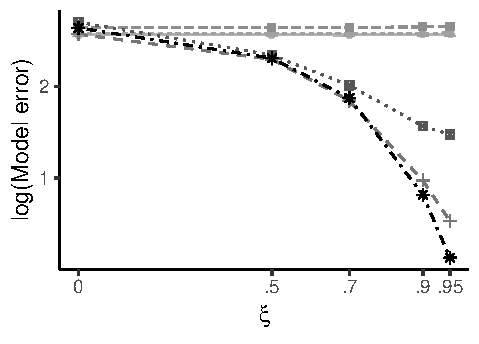
\includegraphics[width=6.5cm]{Plots/NormalHet_AR1_ModelErr_April.pdf} &   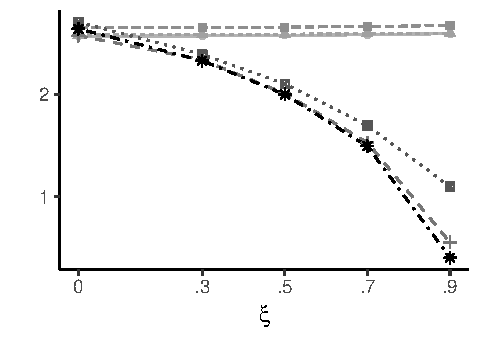
\includegraphics[width=6.5cm]{Plots/NormalHet_Const_ModelErr_April.pdf} & \multirow{4}{*}{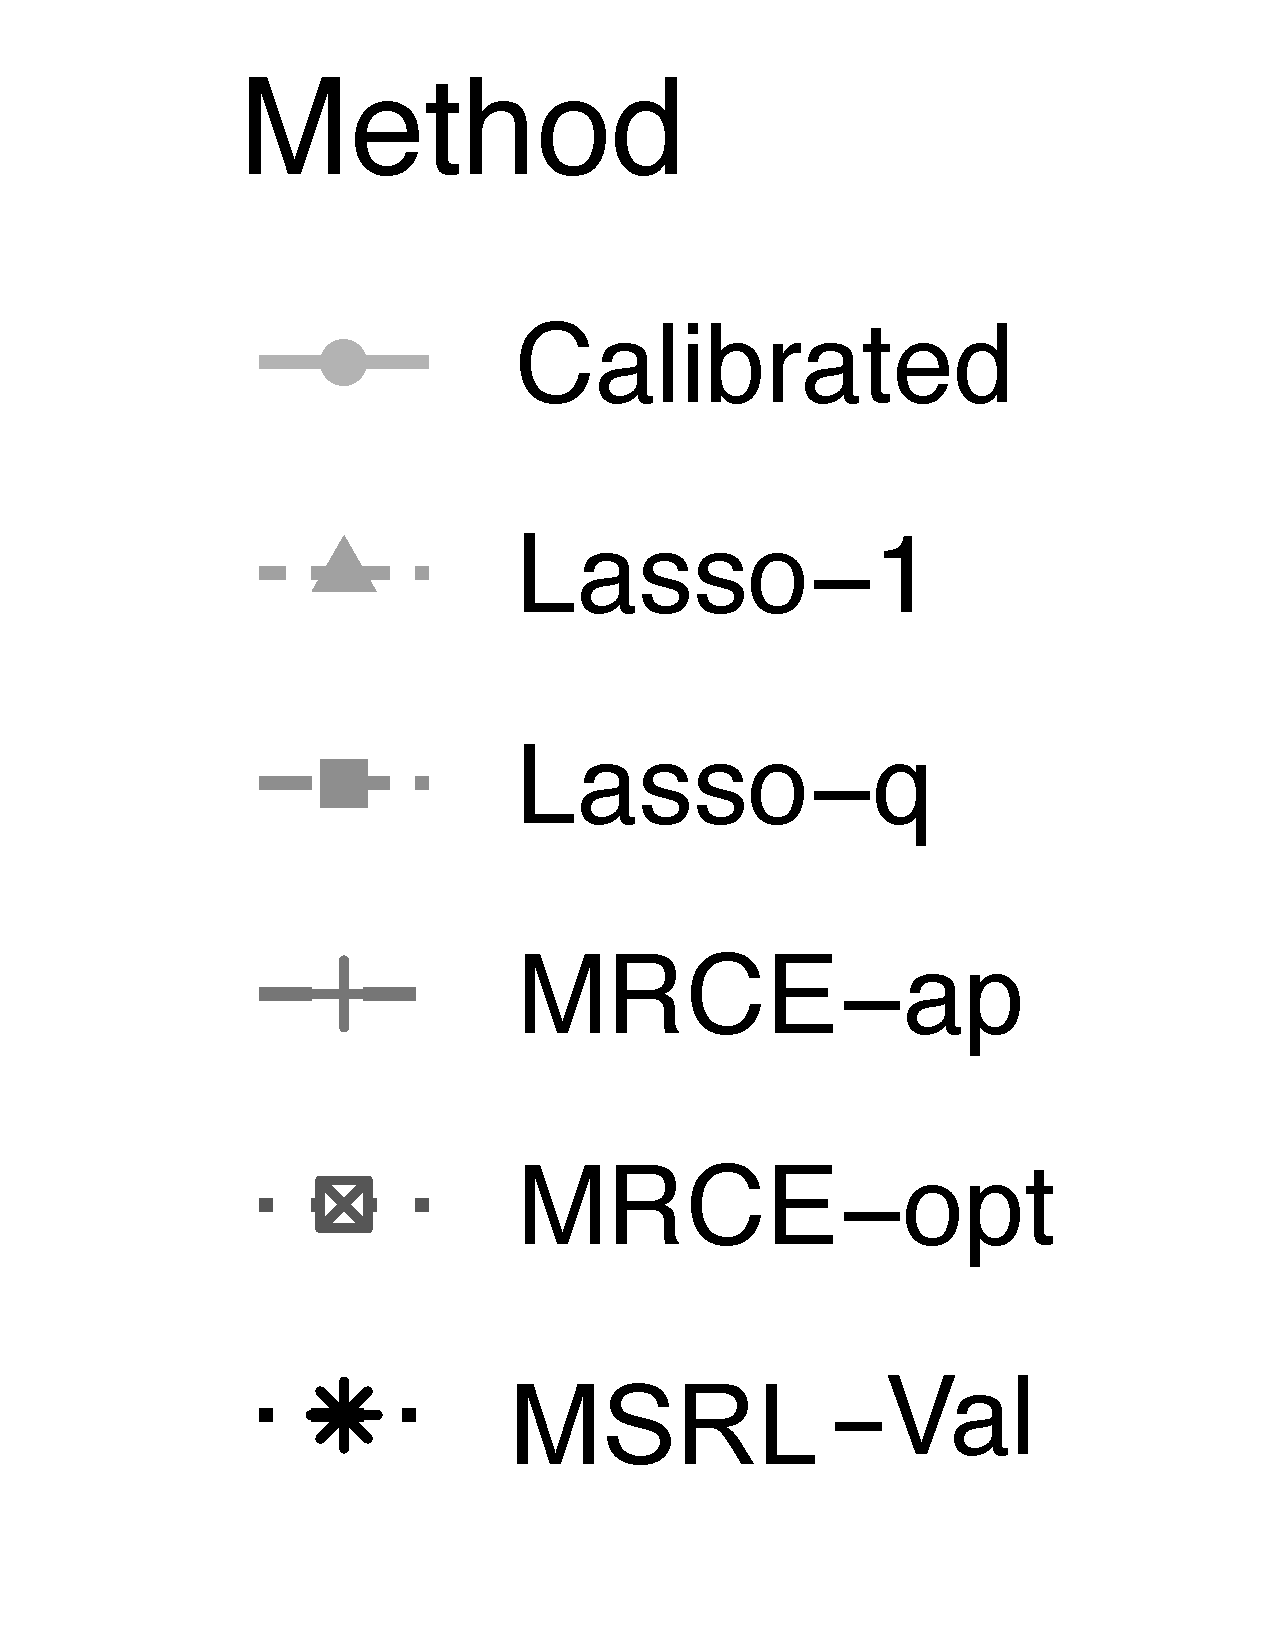
\includegraphics[width=3.5cm]{Plots/Vert_Legend.pdf}} \\
(a) Model 1  & (b) Model 2  & \\[6pt]
 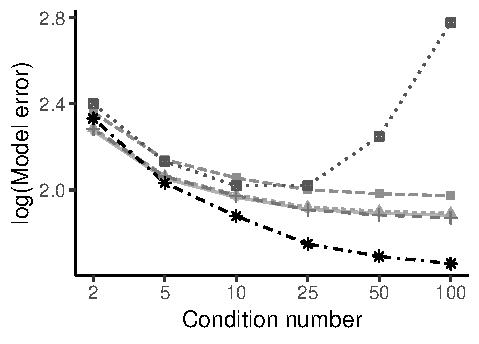
\includegraphics[width=6.5cm]{Plots/NormalHet_Dense_ModelErr_April.pdf} &   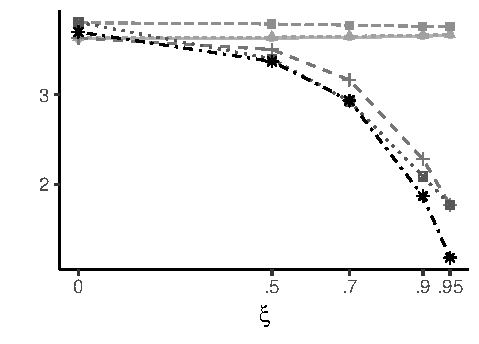
\includegraphics[width=6.8cm]{Plots/THet_AR1_ModelErr_April.pdf} &  \\
(c) Model 3  & (d) Model 4 & \\[6pt]
\end{tabular}
\caption{Average log-model error over one hundred independent replications under Model 1 -- 4 with $\xi$ or $(\rm cond)$ varying and $q=50$.}\label{fig:rho_Results}
\end{figure}

\subsection{Results}\label{subsec:Results}
In Figure \ref{fig:rho_Results} we display the average model error for the six methods we considered. For both Model 1 and Model 2, when $\xi = 0$, the best performing method in terms of model error was \texttt{Calibrated}. This is not surprising since these settings conform to the model assumptions of \citet{liu2015calibrated}. Of our method and the two versions of the method of \citet{rothman2010sparse}, \texttt{MRCE-ap} performed best when $\xi=0$. When the error correlation was high or when $\Sigma_*$ had condition number greater than five, our method outperformed all competitors in terms of model error. In general, \texttt{MSRL-Val} tended to perform similarly to \texttt{MRCE-ap}, which requires the selection of two tuning parameters and is much more computationally intensive. Under Models 1 -- 3, both \texttt{MRCE-ap} and \texttt{MSRL-Val} outperformed \texttt{MRCE-opt}, the penalized maximum likelihood estimator of $\beta_*$ which has oracle knowledge of $\Omega_*$. Under Model 4, where the multivariate normality assumption of both \texttt{MRCE} variants is violated, we see \texttt{MRCE-opt} outperformed \texttt{MRCE-ap}, both of which were outperformed by \texttt{MSRL-Val} as $\xi$ increases. 


In the Supplementary Material, we display weighted prediction error for the same settings displayed in Figure \ref{fig:rho_Results}. The relative performances were similar to those in Figure \ref{fig:rho_Results} -- with \texttt{MSRL-Val} outperforming all competitors when the error correlations were high and when $\Sigma_*$ was moderately ill-conditioned. In addition, we also display both model error and weighted prediction error under Models 1 and 2 with $\xi = 0.9$ and $q$ taking values in $\left\{25, 50, 100, 150\right\}$. We found that as $q$ increased, \texttt{MSRL-Val} and \texttt{MRCE-ap} tended to perform more similarly, with \texttt{MSRL-Val} outperforming \texttt{MRCE-ap} when $q = 25$, but with the two displaying similar performance when $q = 150$.

\begin{table}[t!]
    \begin{adjustwidth}{-.7in}{-1in}  
\scalebox{0.75}{
\begin{tabular}{|c||ccccc|ccccc||ccccc|ccccc|}
  \hline
  & \multicolumn{10}{c||}{Model 1}& \multicolumn{10}{c|}{Model 2}\\ 
  \hline
  & \multicolumn{5}{c|}{TPR} &  \multicolumn{5}{c||}{FPR ($\times 100$)} & \multicolumn{5}{c|}{TPR} &  \multicolumn{5}{c|}{FPR ($\times 100$)} \\
  \hline
 $\xi$ & 0 & 0.5 & 0.7 & 0.9 & 0.95 & 0 & 0.5 & 0.7 & 0.9 & 0.95 & 0 & 0.3 & 0.5 & 0.7 & 0.9 & 0 & 0.3 & 0.5 & 0.7 & 0.9 \\
  \hline
Calibrated & 1.00 & 1.00 & 1.00 & 1.00 & 1.00 & 4.80 & 4.85 & 4.86 & 4.86 & 4.89 & 1.00 & 1.00 & 1.00 & 1.00 & 1.00 & 4.80 & 4.81 & 4.81 & 4.85 & 4.87 \\ 
  Lasso-1 & 1.00 & 1.00 & 1.00 & 1.00 & 1.00 & 4.74 & 4.77 & 4.75 & 4.77 & 4.83 & 1.00 & 1.00 & 1.00 & 1.00 & 1.00 & 4.74 & 4.75 & 4.76 & 4.78 & 4.78 \\ 
  Lasso-q & 1.00 & 1.00 & 1.00 & 1.00 & 1.00 & 4.12 & 4.14 & 4.10 & 4.19 & 4.25 & 1.00 & 1.00 & 1.00 & 1.00 & 1.00 & 4.12 & 4.12 & 4.15 & 4.18 & 4.29 \\
  MRCE-ap & 1.00 & 1.00 & 1.00 & 1.00 & 1.00 & 4.68 & 5.50 & 5.05 & 4.62 & 4.56 & 1.00 & 1.00 & 1.00 & 1.00 & 1.00 & 4.68 & 5.88 & 5.73 & 5.55 & 5.51 \\
  MRCE-opt & 1.00 & 1.00 & 1.00 & 1.00 & 1.00 & 5.93 & 5.11 & 3.99 & 2.03 & 1.43 & 1.00 & 1.00 & 1.00 & 1.00 & 1.00 & 5.93 & 5.72 & 5.31 & 4.34 & 2.27 \\
  \hline
  MSRL-Asymp & 0.70 & 0.76 & 0.84 & 0.95 & 0.98 & 0.00 & 0.00 & 0.00 & 0.00 & 0.00 & 0.70 & 0.79 & 0.88 & 0.95 & 0.99 & 0.00 & 0.00 & 0.00 & 0.00 & 0.00 \\
  MSRL-Asymp-2 & 1.00 & 1.00 & 1.00 & 1.00 & 1.00 & 0.82 & 0.84 & 0.85 & 0.88 & 0.88 & 1.00 & 1.00 & 1.00 & 1.00 & 1.00 & 0.82 & 0.82 & 0.82 & 0.82 & 0.82 \\
  MSRL-Val & 1.00 & 1.00 & 1.00 & 1.00 & 1.00 & 4.54 & 4.47 & 4.44 & 4.43 & 4.52 & 1.00 & 1.00 & 1.00 & 1.00 & 1.00 & 4.54 & 4.55 & 4.56 & 4.59 & 4.68 \\ 
 MSRL-q95 & 0.89 & 0.93 & 0.97 & 1.00 & 1.00 & 0.00 & 0.00 & 0.00 & 0.00 & 0.00 & 0.89 & 0.95 & 0.98 & 1.00 & 1.00 & 0.00 & 0.00 & 0.00 & 0.00 & 0.00 \\ 
  MSRL-q95-2 & 1.00 & 1.00 & 1.00 & 1.00 & 1.00 & 1.65 & 1.68 & 1.70 & 1.73 & 1.73 & 1.00 & 1.00 & 1.00 & 1.00 & 1.00 & 1.65 & 1.66 & 1.65 & 1.66 & 1.66 \\
   \hline
\end{tabular}
}
 \end{adjustwidth}
\caption{Average true positive and false positive (times 100) rates for identifying nonzero entries in $\beta_*$. }\label{table:TPRFNR}
\end{table}

\subsection{Theoretical tuning results}\label{subsec:TP_sel}
Based on our theoretical results, we also studied selecting tuning parameters for \eqref{eq:MSRL} in two more computationally efficient ways: (i) based on quantiles of the empirical distribution of the random variable $\frac{c}{\sqrt{n}}\|X'O^{(n)}_q\|_{\rm max}$ where $O$ is a random matrix whose distribution is uniform over the set of $n \times q$ orthogonal matrices (i.e., $O^{(n)}_q$ such that ${O^{(n)}_q}'O^{(n)}_q = I_q$) and (ii) based on the analytic expression from Theorem 1. We used these approaches with $\xi$ varying for Models 1 and 2.  Note that these approaches require fitting \eqref{eq:MSRL} for only a single tuning parameter, and thus, are far more computationally efficient than any of the competing methods.

To approximate the distribution of the random variable used in (i), we generated 10,000 orthogonal matrices $O^{(n)}_q$ independently by generating $U \in \mathbb{R}^{n \times q}$ whose entries are iid ${\rm N}(0,1)$ and setting $O^{(n)}_q = U(U'U)^{-1/2}$ \citep{eaton}. 

We tried three versions of the two tuning approaches: \texttt{MSRL-q95} sets $\lambda$ equal to the 95th quantile of the empirical distribution of $\frac{1.01}{\sqrt{n}}\|X'O^{(n)}_q\|_{\rm max}$. Like \citet{belloni2011square}, we found \texttt{MSRL-q95} performed well at variable selection, often having a false positive rate of zero. However, like \citet{belloni2011square}, we also found that this choice of $\lambda$ led to substantial bias. Thus, we also used \texttt{MSRL-q95-RF}, a refitted version of \texttt{MSRL-q95} where we re-estimate the coefficients using a likelihood-based seemingly unrelated regression estimator described in the Supplementary Material. In addition to the refitted estimator, we also consider a version which the $95$th quantile tuning parameter times one-half, which we call \texttt{MSRL-q95-2}. We also tried variations of \texttt{MSRL} based on the analytic expression for $\lambda$ from Theorem 1. Specifically, for \texttt{MSRL-Asymp}, we use $\lambda = 1.01 \left\{2 n^{-1} \log(2 pq /.05)\right\}^{1/2}$ and repeated the same refitting procedure to obtain \texttt{MSRL-Asymp-RF}. In addition, we use $\lambda = \frac{1.01}{2} \left\{2 n^{-1} \log(2 pq /.05)\right\}^{1/2}$ to obtain \texttt{MSRL-Asymp-2}. 

\begin{figure}[t!]
\centerline{\hfill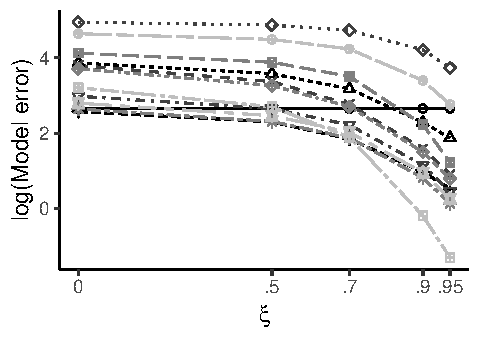
\includegraphics[width=8cm]{Plots/NormalHet_AR1_ModelErr_TP_April.pdf} \hfill 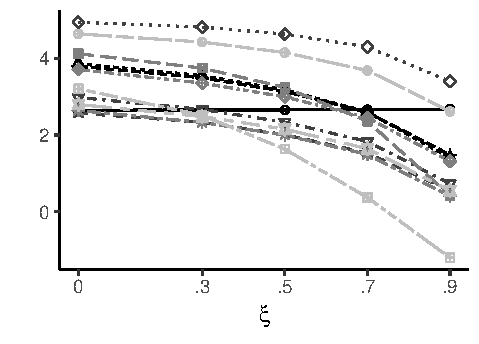
\includegraphics[width=8cm]{Plots/NormalHet_Const_ModelErr_TP_April.pdf}\hfill}
\centerline{\hfill (a) Model 1\hfill \quad \hfill (b) Model 2 \hfill}
\centerline{\hfill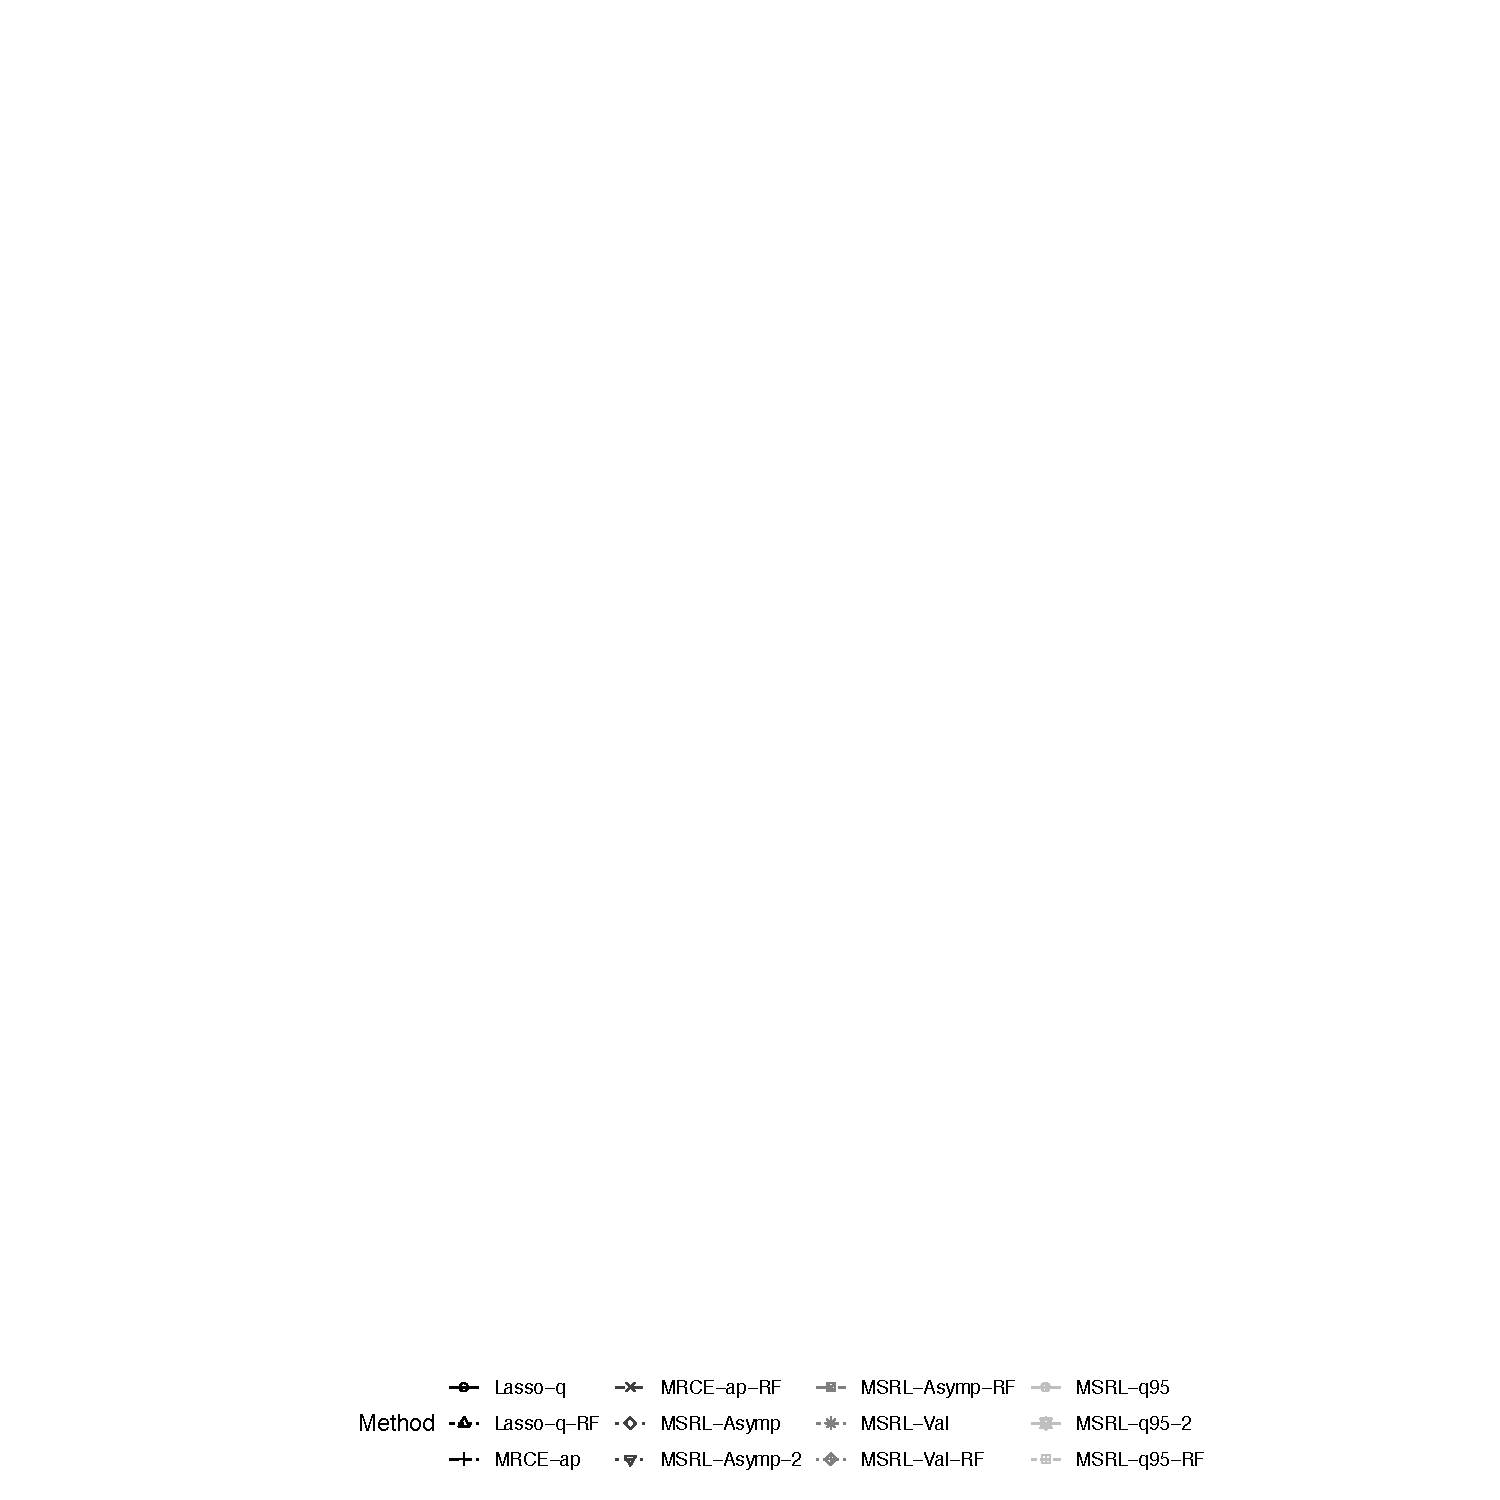
\includegraphics[width=16cm]{Plots/TP_LegendGet.pdf}\hfill} 
\caption{Average log-model error over one hundred independent replications under Model 1 - 2 with $\xi$ varying.}\label{fig:TP_Results}
\end{figure}


Model error averages (on the log scale) for these approaches are displayed in Figure \ref{fig:TP_Results}. Average true positive and false positive rates are displayed in Table \ref{table:TPRFNR}. As observed in \citet{belloni2011square}, the theory-based tuning parameters selected smaller models than validation-based tuning parameters. In particular, when $\xi > .70$, the tuning parameter based on the quantiles of $\frac{1.01}{\sqrt{n}}\|X'O^{(n)}_q\|_{\rm max}$ had nearly perfect variable selection accuracy, whereas the validation based approach tended to include many irrelevant predictors. However, refitting appears necessary to counterbalance the additional bias incurred from using the nuclear norm as a loss function -- a conclusion also drawn by \citet{belloni2011square}. Both versions of \texttt{MSRL} which use one-half times the theory-based tuning parameter values tended to perform similar to the validation-based version \texttt{MSRL-Val}. Together, these results suggest that theory-based tuning could be a useful alternative to validation-based tuning when variable selection accuracy and computational efficiency are priorities. 

% \begin{figure}[!htbp]
% \centerline{
% \hfill\includegraphics[width=6.6cm]{Plots/NormalHet_AR1_ME.pdf}\hfill
% \includegraphics[width=10.8cm]{Plots/NormalHet_AR1_PE.pdf}\hfill}
% %\centerline{\hfill\makebox[7.5cm]{(a)}\hfill\makebox[7.5cm]{(b)}\hfill}
% \centerline{
% \hfill\includegraphics[width=6.3cm]{Plots/NormalHet_Const_ME.pdf}\hfill
% \includegraphics[width=10.5cm]{Plots/NormalHet_Const_PE.pdf}\hfill}
% %\centerline{\hfill\makebox[width=5]{(c)}\hfill\makebox[width=5]{(b)}\hfill}
% \caption{Model error and prediction error for the six candidate methods over one hundred independent replications under Model 2.}\label{fig:Model1_Results}
% \end{figure} 

\section{Glimoblastoma multiforme application}
We used our method to model the linear relationship between microRNA expression and gene expression in patients with glimoblastoma multiforme, a brain cancer, collected by the Cancer Genome Atlas Project (TCGA, \citet{weinstein2013cancer}). We were motivated to apply our method to these data as earlier versions of this dataset were analyzed by \citet{wang2015joint} and \citet{lee2012simultaneous}, both of whom proposed new methods for multivariate response linear regression which explicitly modelled the error precision matrix. Following both \citet{wang2015joint} and \citet{lee2012simultaneous}, mircoRNA expression profiles were treated as the response and gene expression profiles were treated as predictors. The preprocessed data were obtained using the \texttt{TCGA2STAT} R package \citep{wan2015tcga2stat}: gene expression data was measured on an Agilent 244K Custom Gene Expression G4502A-07 microarray and microRNA were measured on an Agilent 8x15K Human miRNA-specific microarray. 

Following \citet{wang2015joint}, we first reduced the dimensionality of both predictors and responses, keeping the $g$ genes with largest median absolute deviation and the $m$ microRNAs with largest median absolute deviation.  We then removed 93 subjects whose first two principal components for gene expression were substantially different than the majority of subjects: after removing these patients, there were 397 subjects in our complete dataset. An R script for creating the datasets we analyzed is available at \href{http://github.com/ajmolstad/MSRL}{github.com/ajmolstad/MSRL}. 

For one hundred independent replications, we randomly split the data into training and testing sets of size 250 and 147 respectively. We fit the multivariate response regression model using four separate methods described in Section \ref{subsec:comp_methods}: \texttt{MSRL-Val}, \texttt{Lasso-q}, \texttt{Lasso-1}, and a variation of \texttt{MRCE-ap}. For \texttt{MSRL-Val}, \texttt{Lasso-q}, and \texttt{Lasso-1}, tuning parameters are selected by five fold cross validation minimizing prediction error. Unfortunately, computing times for \texttt{MRCE-ap} could be extremely long, so we tried ``best-case'' tuning, i.e., we select the tuning parameters which gives the minimum prediction error on the test set. Note that this approach is not applicable in practice, but is included to demonstrate that \texttt{MSRL-Val} performs similarly to the much more computationally intensive approach. For comparison, we also include the ``best-case'' tuning version of \texttt{MSRL}.  We denote both of these versions with a superscript $*$ in Table \ref{table:TCGA}.

\begin{table}[t!]
\centering
\begin{tabular}{|c|cc|cc|cc|cc|}
  \hline
  & \multicolumn{4}{c|}{Weighted prediction error} & \multicolumn{4}{|c|}{Nuclear norm prediction error} \\
  \hline
$m$ & \multicolumn{2}{c|}{20} & \multicolumn{2}{c|}{40} & \multicolumn{2}{c|}{20} & \multicolumn{2}{c|}{40} \\
$g$ &  500 & 1000 & 500 & 1000 & 500 & 1000 & 500 & 1000 \\ 
  \hline
   \texttt{MSRL-Val} & 0.6424 & 0.6103 & 0.6698 & 0.6435 & 0.2128 & 0.2069 & 0.3388 & 0.3317 \\ 
 \texttt{Lasso-1}  & 0.6518 & 0.6164 & 0.6747 & 0.6442 & 0.2146 & 0.2086 & 0.3403 & 0.3329 \\ 
   \texttt{Lasso-q} & 0.6518 & 0.6167 & 0.6764 & 0.6455 & 0.2148 & 0.2088 & 0.3422 & 0.3347 \\ 
   \hline
   \hline
   \texttt{MSRL}$^*$ & 0.6413 & 0.6073 & 0.6690 & 0.6413 & 0.2127 & 0.2068 & 0.3387 & 0.3319 \\ 
  \texttt{MRCE-ap}$^*$ & 0.6416 & 0.6060 & 0.6659 & 0.6354 & 0.2130 & 0.2069 & 0.3387 & 0.3314 \\ 
  \hline
\end{tabular}
\caption{Weighted prediction error and nuclear norm prediction error averaged over 100 training/testing splits for the five considered methods. }\label{table:TCGA}
\end{table}



We compared the five methods in terms of two prediction metrics: weighted prediction error, $\|(Y_{\rm test} - \hat{Y}_{\hat{\beta}}) \Lambda^{-1}\|_F^2/147 m$ and nuclear-norm prediction error, $\|Y_{\rm test} - \hat{Y}_{\hat{\beta}}\|_*/1000$; where $\Lambda$ is a diagonal matrix with the complete data response standard deviations along its diagonal. For \texttt{Lasso-1} and \texttt{Lasso-q}, we standardized the response variables for model fitting whereas for our method, we instead weighted the $\ell_1$-norm penalty by the response standard deviations. For \texttt{MRCE-ap}$^*$, we standardized response variables so that the precision matrix estimate was on the correlation scale. 

In Table \ref{table:TCGA}, we display prediction errors averaged over 100 replications in the various settings. Amongst the methods which could be used in practice, \texttt{MSRL-Val} substantially outperformed both \texttt{Lasso-1} and \texttt{Lasso-q} in terms of weighted prediction error when $g = 500$. When $g = 1000$, \texttt{MSRL-Val} performed only slightly better than either \texttt{Lasso} variant. Both ``best-case'' methods performed slightly better than \texttt{MSRL-Val}, with the more computationally intensive \texttt{MRCE-ap}$^*$ slightly outperforming \texttt{MSRL}$^*$ in the higher-dimensional settings. In terms of nuclear norm prediction error, \texttt{MSRL-Val} outperformed both \texttt{Lasso} variants in every setting, and even performs better than \texttt{MRCE-ap}$^*$ in some settings. 

\section{Discussion}
In this article, we study the multivariate square-root lasso from theoretical, computational, and empirical perspectives. However, there are a number of important directions for future research, which we outline here. First, additional work is needed to understand the asymptotic behavior of estimates of $\beta_*$ based on the refitting procedure used in Section \ref{sec:sim_studies}. In particular, because ordinary least squares fails to account for dependent errors, the refitting procedure we employ explicitly estimates the error precision matrix. When $q$ is large, this approach may be infeasible or may perform poorly due to ill-conditioning of the error precision matrix. 

Second, the prox-linear ADMM algorithm we propose in Section 3.2 could also be applied to a broad class of penalized regression estimators which use non-differentiable loss functions, e.g., using the $\ell_1$-norm as in least absolute deviation regression \citep{WANG2013135}, or a generalization using the matrix 1-norm. 

Finally, because \eqref{eq:MSRL} is convex and does not require an estimate of the error covariance matrix to account for dependent errors, \eqref{eq:MSRL} is a reasonable alternative to some existing methods, e.g., \citet{rothman2010sparse} or \citet{yin2011sparse} when an estimate of the precision matrix is not needed. However, even if an estimate of the error covariance or precision matrix is also desired by the practitioner, Remark 1 suggests that the estimate obtained by solving \eqref{eq:MSRL} may perform reasonably well in certain settings. Unfortunately, when $q$ is large, there is no guarantee that this estimate will be positive definite. Hence, one may consider using \eqref{eq:joint_interp} after introducing an additional positive definiteness constraint on the optimization variable corresponding to $\Sigma_*$. 

\bibliography{NN_MRR}




\clearpage

\setcounter{page}{1}
\setcounter{section}{0}

\title{Supplementary Material for ``Insights and algorithms for the multivariate square-root lasso''}

\maketitle%2
\section{Proofs of Proposition 1 and Theorem 1}
We first provide a number of lemmas which will be useful for establishing results throughout the manuscript. For ease of notation, we use $\kappa$ in place of $\kappa_{\mathcal{E}, c}.$ Recall $\bar{c} = (c+1)/(c-1)$ and $\|A\| = \varphi_1(A)$ where $\varphi_j(A)$ is the $j$th largest singular value of $A$. Let $\sum_{j,k}|\beta_{j,k}| \equiv |\beta|_1, \sum_{(j,k) \in \mathcal{S}}|\beta_{j,k}| \equiv |\beta_{\mathcal{S}}|_1,$ and $\sum_{(j,k) \notin \mathcal{S}}|\beta_{j,k}| \equiv |\beta_{\mathcal{S}^c}|_1$. 

We first state a result from \citet{eaton}, which will be used throughout our proofs. This statement follows immediately from their proof of their Proposition 7.1. 
\begin{lemma}(\citet{eaton})\label{lemma:eaton}
Suppose $Z \in \mathbb{R}^{n \times q}$ is a random matrix which has $q$ singular values almost surely and suppose $Z$ is left-spherical, i.e., for any $n \times n$ orthogonal matrix $O_n^{(n)}$, $O_n^{(n)} Z$ has the same matrix variate distribution as $Z$. Let $U_Z D_Z V_Z' = {\rm svd}(Z)$. Then, $Z(Z'Z)^{-1/2}  = U_Z V_Z'$ follows a uniform distribution of the set of $n \times q$ semiorthogonal matrices, i.e., the set of matrices $W_q^{(n)} \in \mathbb{R}^{n \times q}$ such that ${W_q^{(n)}}'W_q^{(n)} = I_q$.
\end{lemma}

\begin{lemma}\label{lemma:grad}
Assume A1 is true. Then, the subgradient of $\|Y - X\beta_*\|_*$ is 
$$ \nabla_\beta \|Y - X\beta_*\|_* =  - X'U_* V_*' = - X'(Y - X\beta_*)[(Y - X\beta_*)'(Y- X\beta_*)]^{-\frac{1}{2}}$$
where $U_* D_* V_*' = {\rm svd}(Y - X\beta_*).$
\end{lemma}
\noindent \textit{Proof of Lemma \ref{lemma:grad}.} When $(Y- X\beta_*)$ has $q$ nonzero singular values, we can write 
\begin{align*} 
(Y - X\beta_*)[(Y - X\beta_*)'(Y- X\beta_*)]^{-\frac{1}{2}} = U_* D_* V_*'(V_* D_* U_*'U_* D_* V_*' )^{-\frac{1}{2}}  = U_* V_*' 
\end{align*}
Thus, we only need to verify the first equality. We proceed with the following steps: first, we derive the subgradient for $\|Y - X\beta_*\|_*$, then we show that the subgradient contains only a single element when $(Y - X\beta_*)$ has $q$ nonzero singular values. Let $\partial_X f(X)$ denote the subgradient of $f$ with respect to $X$. 


To establish the subgradient, we first apply the chain rule for subdifferentials:
\begin{equation}\label{eq:partial1}
\partial_\beta \|Y - X\beta\|_* = \left\{ - X'H: H \in \partial_B \|B\|_*\mid_{B = Y - X\beta} \right\}.
\end{equation} 
From \citet{watson1992characterization}, letting $U_BD_BV_B' = {\rm svd}(B)$, we have 
\begin{equation}\label{eq:partial2}
 \partial_B\|B\|_* = \left\{UV' + W: W \in \mathbb{R}^{p \times q}, \|W\|\leq 1, U_B'W = 0, W V_B = 0 \right\}.
 \end{equation}
Hence, combining \eqref{eq:partial1} and \eqref{eq:partial2},
$$ \partial_\beta \|Y - X\beta\|_*  = \left\{ -X'U_\beta V_\beta' - X'W:  \|W\|\leq 1, U_\beta'W = 0, W V_\beta = 0\right\}.$$
However, by the rank-nullity theorem, when $Y - X\beta_*$ has $q$ nonzero singular values (i.e., is full column rank), the only such $W$ which can satisfy both $U_\beta'W = 0$ and $W B_\beta = 0$ is $W = 0$. Thus, in this case, the subgradient is a single point so can write
$\nabla_\beta \|Y - X\beta_*\|_* = - X'U_* V_*'$ where $U_* D_* V_*' = {\rm svd}(Y - X\beta_*). \quad\quad \blacksquare$

\bigskip
% In the following lemmas, we refer to the $\ell_1$-penalized version of \eqref{eq:MSRL}. 

\begin{lemma}\label{RSClemma}
Assume A1 is true. Then, for all $\Delta \in \mathcal{C}(\mathcal{S}, c)$, 
$$ \frac{1}{\sqrt{n}}\|Y - X\beta_* - X\Delta\|_* - \frac{1}{\sqrt{n}}\|Y - X\beta_*\|_* \geq \kappa \|\Delta\|_F^2 - \frac{1}{\sqrt{n}}{\rm tr}(\Delta'X'U_*V_*')$$
where $U_*D_*V_*' = {\rm svd}(Y - X\beta_*)$. 
\end{lemma}
\noindent \textit{Proof of Lemma \ref{RSClemma}.} First, recall that the nuclear norm can be equivalently written 
$$ \|A\|_* = \sup_{\|Q\| \leq 1} {\rm tr}(Q'A).$$
Also recall that for any convex function $f$, 
$\mathcal{L}(\beta_*, \Delta) = f(\beta_* + \Delta) - f(\beta_*) - {\rm tr}\left\{ \nabla_\beta f(\beta_*)'\Delta\right\} \geq 0.$ 
Hence, letting $f(\beta_*) = \frac{1}{\sqrt{n}} \|Y - X\beta_*\|_*$ and using that $\nabla_\beta f(\beta_*) = -\frac{1}{\sqrt{n}}X'U_*V_*'$ under A1 by Lemma \ref{lemma:grad}, we want to show
$$\mathcal{L}(\beta_*, \Delta) = \frac{1}{\sqrt{n}}\|Y - X\beta_* - X\Delta\|_* - \frac{1}{\sqrt{n}}\|Y - X\beta_*\|_*  + \frac{1}{\sqrt{n}}{\rm tr}(\Delta'XU_*V_*')  \geq \kappa \|\Delta\|_F^2. $$
Notice, using the dual definition of the nuclear norm, 
\begin{align}
\mathcal{L}(\beta_*, \Delta) & = \sup_{\|Q_1\| \leq 1} \frac{1}{\sqrt{n}}{\rm tr}\left\{ Q_1'(U_*D_*V_*' - X\Delta)\right\} - \sup_{\|Q_2\| \leq 1}\frac{1}{\sqrt{n}} {\rm tr}(Q_2'U_*D_*V_*')  + \frac{1}{\sqrt{n}}{\rm tr}(\Delta'XU_*V_*')\notag
\intertext{and the $Q_2$ that maximizes the second term is $Q_2 = U_*V_*'$ by the definition of the nuclear norm, so}
& = \sup_{\|Q_1\| \leq 1} \frac{1}{\sqrt{n}} {\rm tr}\left\{ Q_1'(U_*D_*V_*' - X\Delta)\right\} - \frac{1}{\sqrt{n}}{\rm tr}(V_* U_*'U_*D_*V_*')  + \frac{1}{\sqrt{n}}{\rm tr}(\Delta'XU_*V_*') \notag \\
& = \sup_{\|Q_1\| \leq 1}\frac{1}{\sqrt{n}} {\rm tr}\left\{ (Q_1 -  U_*V_*')'(U_*D_*V_*' - X\Delta\right\}\label{A3_cond}
\intertext{where \eqref{A3_cond} the numerator in the definition of $\kappa$. Thus, we have}
& = \sup_{\|Q_1\| \leq 1}  \frac{1}{\sqrt{n}}{\rm tr}\left\{ (Q_1 -  U_*V_*')'(U_*D_*V_*' - X\Delta\right\} \geq \kappa \|\Delta\|_F^2\notag
\intertext{for all $\Delta \in \mathcal{C}(\mathcal{S}, c)$, which establishes the result. $\quad\quad \blacksquare$} \notag
\end{align}

The following lemma is adapted from Lemma 3 of \citet{negahban2012unified}. 

\begin{lemma}\label{lemma:cone}
Suppose A1 is true and $\lambda > \frac{c}{\sqrt{n}} \|X'U_*V_*'\|_{\rm max}$ for a constant $c > 1$. Then, $\hat{\Delta} = \hat{\beta} - \beta_*$ belongs to the set 
$$\mathcal{C}(\mathcal{S}, c) = \left\{ \Delta \in \mathbb{R}^{p \times q}: \bar{c}\hspace{1pt}|\Delta_\mathcal{S}|_1 \geq |\Delta_{\mathcal{S}^c}|_1 \right\}.$$
\end{lemma}
\noindent \textit{Proof of Lemma \ref{lemma:cone}:} Let $f(\beta) = \frac{1}{\sqrt{n}} \|Y - X \beta\|_* + \lambda |\beta|_1.$ Since $\hat{\beta}$ is the minimizer of $f$ and because $f$ is convex, letting $\hat{\Delta} = \hat{\beta} - \beta_*$, we have
\begin{align*}
0 & \geq f(\beta_* + \hat{\Delta}) - f(\beta_*)  \geq  \frac{1}{\sqrt{n}} \|Y - X \beta_* - X\hat{\Delta}\|_* -  \frac{1}{\sqrt{n}} \|Y - X \beta_*\|_* + \lambda |\beta_* + \hat{\Delta}|_1 - \lambda |\beta_*|_1.
\intertext{Recall, because the nuclear norm is convex, its first order Taylor expansion is nonnegative so under A1, by Lemma \ref{lemma:grad} we have $\frac{1}{\sqrt{n}} \|Y - X \beta_* - X\hat{\Delta}\|_* -  \frac{1}{\sqrt{n}} \|Y - X \beta_*\|_*  \geq - \frac{1}{\sqrt{n}} |{\rm tr}(\hat{\Delta}'X'U_*V_*')|$. In addition, by the same argument as in \citet{rothman2008sparse} to obtain equation (11), 
$\lambda |\beta_* + \hat{\Delta}|_1 - \lambda |\beta_*|_1 \geq \lambda(|\hat{\Delta}_{\mathcal{S}^c}|_1 - |\hat{\Delta}_\mathcal{S}|_1)$, so together we have}
0 & \geq  - \frac{1}{\sqrt{n}}|{\rm tr}(\hat{\Delta}'X'U_*V_*')| + \lambda |\beta_* + \hat{\Delta}|_1 - \lambda |\beta_*|_1 \geq  - \frac{1}{\sqrt{n}}|{\rm tr}(\hat{\Delta}'X'U_*V_*')| + \lambda(|\hat{\Delta}_{\mathcal{S}^c}|_1 - |\hat{\Delta}_\mathcal{S}|_1)
 \intertext{Finally, because $|{\rm tr}(\hat{\Delta}'X'U_*V_*')| \leq \|X'U_*V_*'\|_{\rm max} |\hat{\Delta}|_1$, and because $\lambda > \frac{c}{\sqrt{n}} \|X'U_*V_*'\|_{\rm max}$ by assumption }
  0 & \geq  - \frac{1}{\sqrt{n}}\|X'U_*V_*'\|_{\rm max} |\hat{\Delta}|_1 + \lambda(|\hat{\Delta}_{\mathcal{S}^c}|_1 - |\hat{\Delta}_\mathcal{S}|_1) \geq - \frac{\lambda}{c}(|\hat{\Delta}_{\mathcal{S}^c}|_1 + |\hat{\Delta}_{\mathcal{S}}|_1) + \lambda(|\hat{\Delta}_{\mathcal{S}^c}|_1 - |\hat{\Delta}_\mathcal{S}|_1) 
  \intertext{which implies
  $$ \frac{c+1}{c}|\hat{\Delta}_{\mathcal{S}}|_1 \geq \frac{c-1}{c}|\hat{\Delta}_{\mathcal{S}^c}|_1,$$
  the desired inequality. $\quad \quad \blacksquare$
  }
\end{align*}


\begin{lemma}\label{main_lemma}
Assume A1 is true. If $\lambda = \frac{\kappa \epsilon}{\bar{c}\sqrt{s}}$, then $\frac{c}{\sqrt{n}}\|X'U_*V_*'\|_{\rm max} < \lambda$ implies $\|\hat{\beta} - \beta_*\|_F \leq \epsilon$.
\end{lemma}
\textit{Proof of Lemma \ref{main_lemma}.} To prove Lemma \ref{main_lemma}, we follow the proof technique from \citet{rothman2008sparse}, detailed in \citet{negahban2012unified}. Define $\mathcal{B}_{\epsilon, c} = \left\{ \Delta \in \mathbb{R}^{p \times q}: \|\Delta\|_F = \epsilon, \bar{c}\hspace{1pt}|\Delta_\mathcal{S}|_1 \geq |\Delta_{\mathcal{S}^c}|_1 \right\}$. Let $f$ be the objective function in \eqref{eq:MSRL}. Because $f$ is convex and $\hat{\beta}$ is its minimizer, and applying Lemma \ref{lemma:cone}, $$\inf \left\{ f(\beta_* + \Delta) : \Delta \in \mathcal{B}_{\epsilon, c} \right\} > f(\beta_*) \implies \|\hat{\beta} - \beta_*\|_F \leq \epsilon.$$  Let $D(\Delta) = f(\beta_*  + \Delta) - f(\beta_*)$ so that if we can show $D(\Delta) > 0$ for $\Delta \in \mathcal{B}_{\epsilon, c}$, the conclusion follows. First, 
\begin{align}
D(\Delta) & = \underbrace{\frac{1}{\sqrt{n}}\|Y - X\beta_* - X\Delta\|_* - \frac{1}{\sqrt{n}}\|Y - X\beta_*\|_*}_{T_1} + \underbrace{\lambda \left(|\beta_* + \Delta|_1 -  |\Delta|_1 \right)}_{T_2} \notag 
 \intertext{so that using Lemma \ref{RSClemma} to bound $T_1$ and applying the argument from \citet{rothman2008sparse} to obtain (11) to bound bound $T_2$, we have}
 % & \geq \kappa \|\Delta\|_F^2 - \frac{1}{\sqrt{n}}{\rm tr}(\Delta X'UV) + \lambda |\beta_* + \Delta|_1 - \lambda |\Delta|_1 \\
 & \geq \kappa \|\Delta\|_F^2 - \frac{1}{\sqrt{n}}|{\rm tr}(\Delta X'U_*V_*')| + \lambda\left(|\Delta_{\mathcal{S}^c}|_1 - |\Delta_\mathcal{S}|_1\right)\notag\\
&  \geq \kappa \|\Delta\|_F^2 - \frac{1}{\sqrt{n}}|\Delta|_1 \|X'U_*V_*'\|_{\rm max} + \lambda(|\Delta_{\mathcal{S}^c}|_1 - |\Delta_\mathcal{S}|_1) \label{holder}\\
\intertext{where \eqref{holder} follows from H{\"o}lder's inequality. Thus, since $\frac{c}{\sqrt{n}}\|X'UV'\|_{\rm max} < \lambda$ by assumption; and because $|\Delta|_1 = |\Delta_\mathcal{S}|_1 + |\Delta_{\mathcal{S}^c}|_1$ and $|\Delta_\mathcal{S}| \leq \sqrt{s}\|\Delta\|_F$, we have from \eqref{holder}}
% D(\Delta) &  \geq \kappa \|\Delta\|_F^2 - \frac{\lambda}{c} \left(|\Delta_{S^c}|_1 + |\Delta_S|_1 + c|\Delta_{S^c}|_1 - c|\Delta_S|_1\right) \notag \\
% & \geq \kappa \|\Delta\|_* -  \frac{\lambda(c+1)}{c} |\Delta_S|_1\notag \\
D(\Delta) & \geq \kappa \|\Delta\|_* - \lambda\left(\frac{c+1}{c}\right) \sqrt{s}\|\Delta\|_F
\intertext{so that finally, because $\|\Delta\|_F = \epsilon$ for $\Delta \in \mathcal{B}_{\epsilon,c}$,  $\lambda = \frac{\kappa \epsilon}{\bar{c}\sqrt{s}}$ yields}
& = \kappa \epsilon^2 \left\{ 1 -  \lambda \left(\frac{c+1}{c}\right)\frac{\sqrt{s}}{\kappa \epsilon}\right\} =  \kappa \epsilon^2 \left(1 - \frac{c-1}{c}\right) > 0. \quad \quad  \blacksquare \notag
\end{align}
Now, an immediate application of Lemma \ref{main_lemma} yields Proposition 1. 
\medskip

\noindent \textit{Proof of Proposition 1.} To prove the first part of Proposition 1, set $\epsilon = \frac{\bar{c}}{\kappa}\sqrt{s}\lambda$ and apply Lemma \ref{main_lemma}. The second part follows immediately from Lemma \ref{lemma:eaton}, which states that A1 and A2 imply $\mathcal{E}(\mathcal{E}'\mathcal{E})^{-1/2}$ is uniformly distributed on the set of semi-orthogonal matrices. $\quad\quad \blacksquare$
% \begin{lemma}(sara van de geer)\label{lemmaSVDG}
% Let $\eta \sim {\rm N}_n(0, I_n)$ for $n > 2$. For $X \in \mathbb{R}^n$ fixed with $\|X\|_2 = 1$ and for all $0 < t < (n-1)/2$, 
% $$ P\left(\frac{|X'\eta|}{\sqrt{n}\|\eta\|_2} \geq \sqrt{\frac{2t}{n-1}}\right) \leq 2 {\rm exp}(-t).$$
% Restated, for $0 < K < 1,$
% $$ P\left(\frac{|X'\eta|}{\sqrt{n}\|\eta\|_2} \geq K \right) \leq 2 {\rm exp}\{}left\{ - \frac{K^2 (n-1)}{2}\right\}.$$
% \end{lemma}
% The following lemma is from \citet{li2016fast}, combining their equations (A.1), (A.2) and Lemma A.1 from \citet{negahban2012unified}.
\begin{lemma}\label{lemmaFreeLunch}
Let $\alpha \in (0,1)$ and $K > 1$ be fixed constants. Let $\phi_1$ and $\phi_2$ be constants such that $\phi_1^{-1} + \phi_2^{-1} = 1$ and suppose $n \geq \frac{4 K^4}{(K^2 - 1)^2} \log(\phi_2 q/\alpha)$. Suppose $\eta \in \mathbb{R}^n$ has entries which are independent and identically distributed ${\rm N}(0,1)$. Then, for $X \in \mathbb{R}^{n \times p}$ fixed with $\|X_j\|_2 = 1$ for $j=1, \dots, p$, it follows that 
% $$ P\left(\frac{\|X'\eta\|_{\rm max}}{\sqrt{n}\|\eta\|_2} \geq 4 \sqrt{\frac{\log p}{n}} \right) \leq 2p^{-1} + {\rm exp}\left(-\frac{n}{32}\right).$$
% Restated, 
$$ P\left(\frac{1}{\sqrt{n}} \frac{\|X'\eta\|_{\rm max}}{\|\eta\|_2} \geq   K \sqrt{\frac{2\log(2 \phi_1 pq/\alpha)}{n}} \right) \leq \alpha/q .$$
\end{lemma}
\textit{Proof of Lemma \ref{lemmaFreeLunch}.} To prove the inequality, we use the union bound:  $$
P\left(\frac{1}{\sqrt{n}}\frac{\|X'\eta\|_{\rm max}}{\|\eta\|_2} \geq K \sqrt{\frac{2 \log(2 \phi_1 qp/\alpha)}{n}}\right) \leq P\left(\frac{1}{n}\|X'\eta\|_{\rm max} \geq \sqrt{\frac{2\log(2 \phi_1 qp/\alpha)}{n}}\right) + P\left( \frac{\|\eta\|_2}{\sqrt{n}} \leq \frac{1}{K} \right).
$$ %Thus, it suffices to show that both terms in the right hand side are bounded below by $\alpha/2q$. 
Dealing with the first term, for normally distributed random variable $\eta$ and fixed $X$ such that for each $j$, $\|X_j\|_2 = 1$, for $t_1 > 0$,
$$ P\left(\frac{1}{n}\|X'\eta\|_{\rm max} \geq \sqrt{\frac{2 \log(2p) + 2t_1}{n}} \right) \leq {\rm exp}(-t_1),$$
see, for example, Lemma 17.5 of \cite{van2016estimation}.
Thus, letting $t_1 = \log(\phi_1 q/\alpha)$, 
$$ P\left(\frac{1}{n}\|X'\eta\|_{\rm max} \geq  \sqrt{\frac{2\log(2 \phi_1 qp/\alpha)}{n}}\right) \leq \frac{\alpha}{\phi_1q}.$$
In addition, we know from Lemma 1 of \citet{laurent2000adaptive} that for $t_2 > 0$
$$ P\left(\frac{1}{n}\|\eta\|_2^2 \leq 1 - 2\sqrt{\frac{t_2}{n}}\right) \leq {\rm exp}(-t_2),$$
so that setting $t_2 = n\frac{(K^2 - 1)^2}{4K^4} > 0$, we have
$$ P\left( \frac{1}{\sqrt{n}} \|\eta\|_2 \leq \frac{1}{K} \right) = P\left(\frac{1}{n}\|\eta\|_2^2 \leq \frac{1}{K^2} \right)  \leq {\rm exp}\left\{ - n\frac{(K^2 - 1)^2}{4K^4} \right\}.$$
Furthermore, by our assumption on $n$, 
$$ {\rm exp}\left\{ - n\frac{(K^2 - 1)^2}{4K^4} \right\} \leq \frac{\alpha}{\phi_2 q}.$$
Thus, by the union bound, 
\begin{align*} 
P\left(\frac{1}{\sqrt{n}}\frac{\|X'\eta\|_{\rm max}}{\|\eta\|_2} \geq K \sqrt{\frac{2 \log(2 \phi_1qp )}{n}} \right) & \leq P\left(\frac{1}{n}\|X'\eta\|_{\rm max} \geq \sqrt{\frac{2\log(2 \phi_1 qp/\alpha)}{n}}\right) + P\left( \frac{\|\eta\|_2}{\sqrt{n}} \leq \frac{1}{K} \right)  \\
& \leq \alpha/\phi_1 q + \alpha/\phi_2 q = \alpha/q. \quad \quad \blacksquare.
\end{align*}


\begin{lemma}\label{lemmaConc}
Suppose A1 and A2 are true. Let $\tilde{c}$ and $c$ be fixed constants such that $\tilde{c} > c > 1$ and $(\phi_1,\phi_2)$ be fixed constants such that $\phi_1^{-1} + \phi_2^{-1} = 1$. It follows that
$$P\left(\frac{c}{\sqrt{n}}\|X'U_*V_*'\|_{\rm max} \leq  \tilde{c} \sqrt{\frac{2\log(2 \phi_1 pq/\alpha)}{n}}\right) \geq 1 - \alpha,$$
if $n \geq \frac{4 K^4}{(K^2 - 1)^2} \log(\phi_2 q/\alpha)$ with $K = \tilde{c}/c.$
\end{lemma}
\noindent \textit{Proof of Lemma \ref{lemmaConc}}: 
Under Assumptions A1 and A2, by Lemma \ref{lemma:eaton}, $U_*V_*' \in \mathbb{R}^{n \times q}$ is a random matrix uniformly distributed on the set of $n \times q$ orthogonal matrices. Moreover, this fact implies that each column of $O = U_*V_*'$ has a marginal distribution which is uniform on the unit sphere. Thus, by the union bound, we have 
\begin{equation}\label{eq:unionbound} P\left(\frac{1}{\sqrt{n}}\|X'U_*V_*'\|_{\rm max} \geq J\right) \leq  \sum_{k=1}^q P\left(\frac{1}{\sqrt{n}}\|X'O_k\|_{\rm max} \geq J\right).
\end{equation}
Since the $O_k$'s are each uniformly distributed on the unit sphere, we can write $O_k = \gamma_k/\|\gamma_k\|_2$ where $\gamma_k \in \mathbb{R}^{n}$ has entries which are independent and identically distributed ${\rm N(0,1)}.$ Hence, setting $J = \frac{\tilde{c}}{c} \left\{ 2 n^{-1} \log(2\phi_1 pq/\alpha)\right\}^{1/2}$ and applying Lemma \ref{lemmaFreeLunch} to the right hand side of \eqref{eq:unionbound}, we have the result. 

\medskip
\noindent \textit{Proof of Theorem 1}: Let $\dot{c} = \tilde{c}/c$, $\hat{c} = \frac{(c+1)\tilde{c}}{(c-1)}$ and let $\phi_1^{-1} + \phi_2^{-1} = 1$.  Suppose that  $(1-\dot{c}^2)^2 n \geq 4 \dot{c}^4 \log (\phi_2 q/\alpha)$. Set $\epsilon = \frac{\bar{c}}{\tilde{c}\kappa}\sqrt{\frac{2s\log(2 \phi_1 pq/\alpha)}{n}}$ and $\lambda = \tilde{c} \left\{n^{-1}(2\log(2 \phi_1 pq/\alpha) \right\}^{1/2}$. Then, applications of Lemma \ref{main_lemma} and Lemma \ref{lemmaConc} implies
\begin{align*} 
P\left(\|\hat{\beta} - \beta_*\|_F \leq \frac{\hat{c}}{\kappa} \sqrt{\frac{2\log(2 \phi_1 pq/\alpha)}{n}}\right) &\geq P\left(\frac{c}{\sqrt{n}}\|X'U_*V_*'\|_{\rm max} \leq \tilde{c} \left[ n^{-1}\left\{ 2s\log(2 \phi_1 pq/\alpha) \right\} \right]^{1/2} \right)\\
& \geq 1 - \alpha. 
\intertext{Finally, setting $\phi_1 = \phi/(\phi-1)$ and $\phi_2 = \phi$ yields the result. $\quad \quad  \blacksquare$}
\end{align*}
\section{Additional simulation results}
\subsection{Weighted prediction error results}
A second performance metric we consider is weighted prediction error: 
$$\|\Omega_*^{1/2}(Y_{\rm test} - \hat{Y}_{\hat{\beta}})\|^2_F/n_{\rm test}q,$$
where $Y_{\rm test} \in \mathbb{R}^{n_{\rm test} \times q}$ is the testing set of responses and $\hat{Y}_{\hat{\beta}}$ are the predicted values of $Y_{\rm test}$ based on estimate $\hat{\beta}$. The two error metrics (model error and weighted prediction error) are distinct: model error measures how well $\hat{\beta}$ estimates the conditional mean of the response, whereas weighted prediction error measures prediction accuracy in terms of realizations of the response. 

In Figure \ref{fig:predErr_Results}, we display average weighted prediction errors for the six methods under the same settings as in Figure \ref{fig:rho_Results}. As with model error, we saw that the methods were effectively indistinguishable when $\xi$ was small or the condition number was less than 5, but as both $\xi$ and the condition number increase, \texttt{MSRL-Val} tended to outperform competitors. As with model error, \texttt{MRCE-ap} also tended to perform relatively well under Models 1 and 2, but less so under Model 3 and 4. 


\begin{figure}[t!]
\begin{tabular}{ccc}
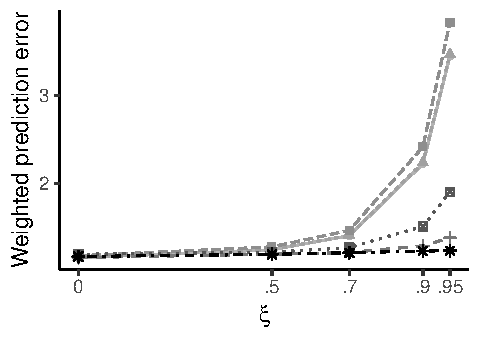
\includegraphics[width=6.9cm]{Plots/NormalHet_AR1_PredErr_April.pdf} &   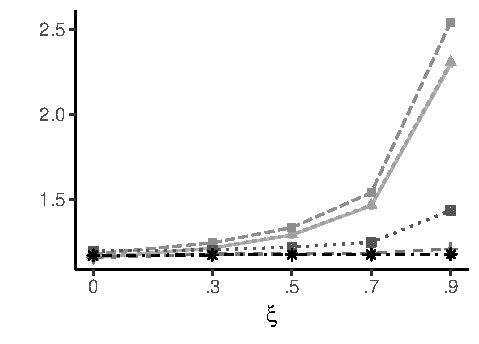
\includegraphics[width=6.9cm]{Plots/NormalHet_Const_PredErr_April.pdf} & \multirow{4}{*}{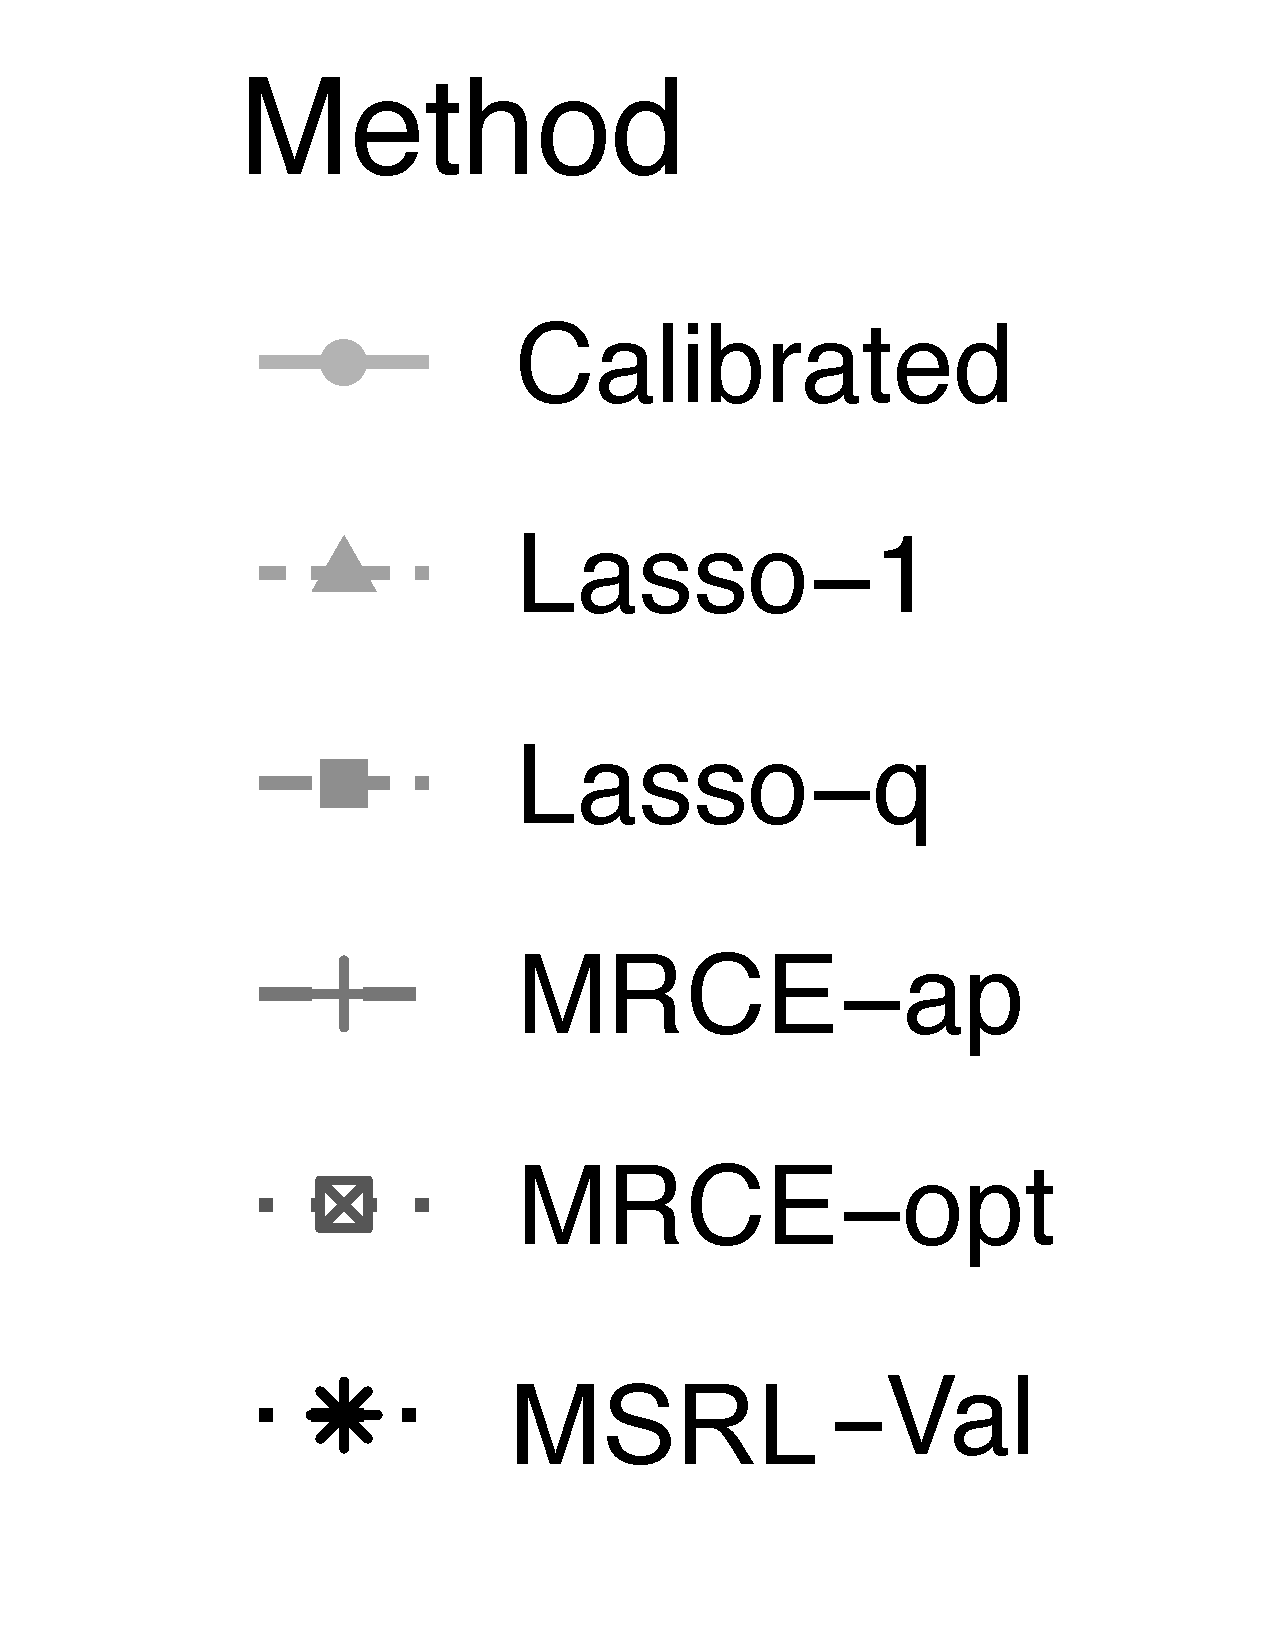
\includegraphics[width=2.5cm]{Plots/Vert_Legend.pdf}} \\
(a) Model 1  & (b) Model 2  & \\[6pt]
 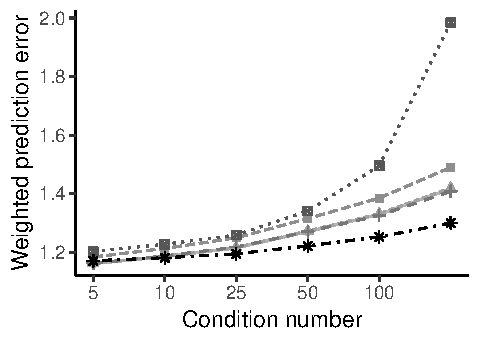
\includegraphics[width=6.9cm]{Plots/NormalHet_Dense_PredErr_April.pdf} &   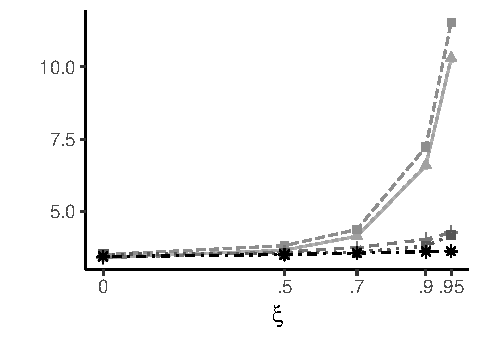
\includegraphics[width=7.1cm]{Plots/THet_AR1_PredErr_April.pdf} &  \\
(c) Model 3  & (d) Model 4 & \\[6pt]
\end{tabular}
\caption{Average weighted prediction error over one hundred independent replications under Model 1 - 4 with $\xi$ or $(\rm cond)$ varying and $q=50$.}\label{fig:predErr_Results}
\end{figure} \


\subsection{Model 1 and 2 with $q$ varying}
In this section, we display additional results from the simulation studies described in Section \ref{sec:sim_studies}. Under the settings of Model 1 and 2, we fit $\xi = 0.9$ and let $q \in \left\{25, 50, 100, 150\right\}$. 
\begin{figure}[t!]
\begin{tabular}{ccc}
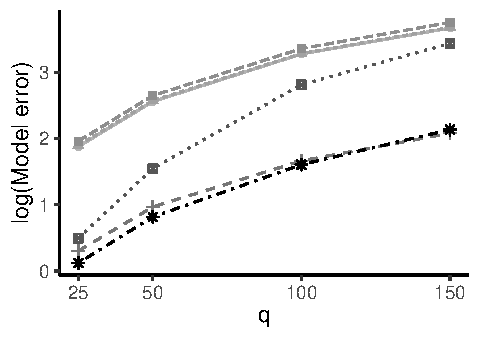
\includegraphics[width=6.5cm]{Plots/NormalHet_qAR1_ModelErr_April.pdf} &   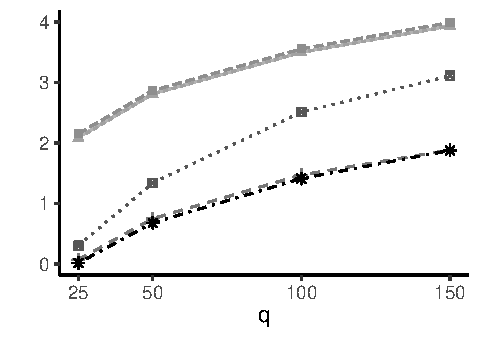
\includegraphics[width=6.5cm]{Plots/NormalHet_qConst_ModelErr_April.pdf} & \multirow{4}{*}{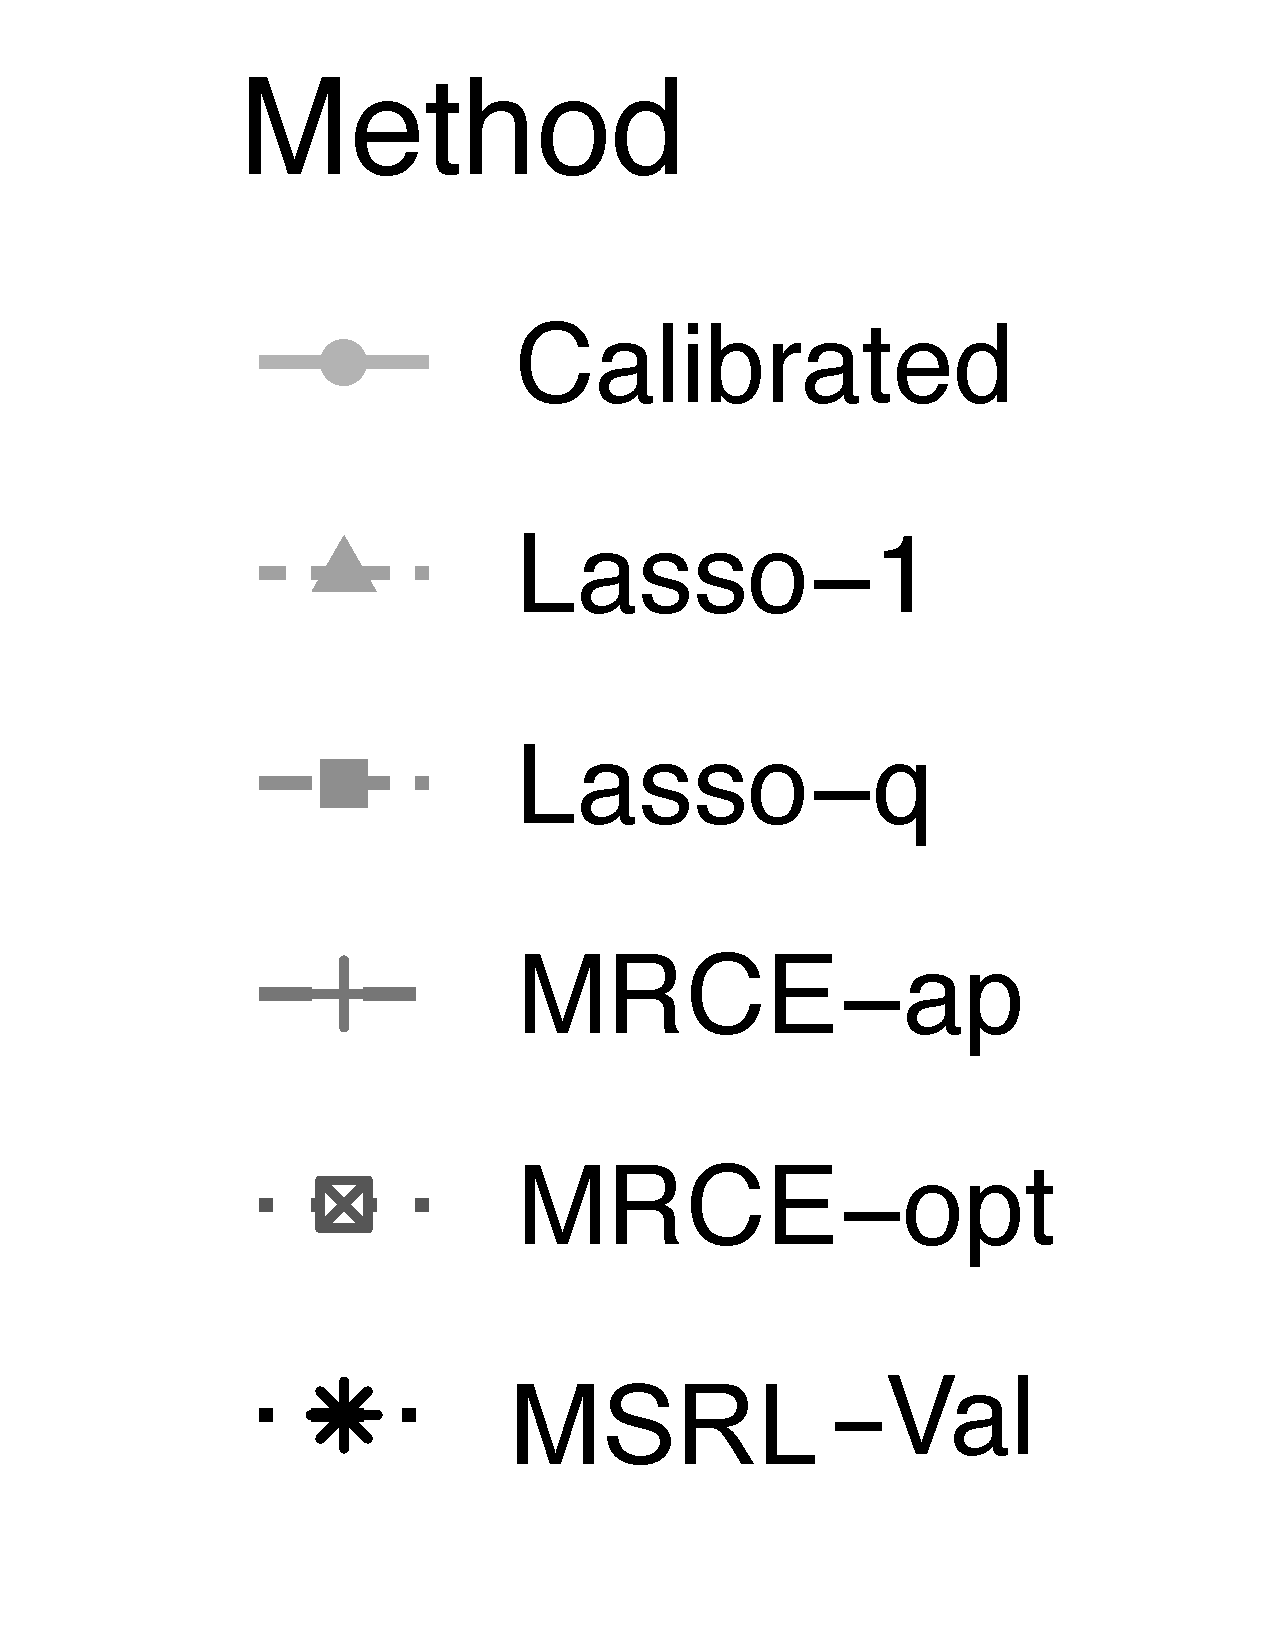
\includegraphics[width=2.5cm]{Plots/Vert_Legend.pdf}} \\
(a)  & (b)  & \\[6pt]
 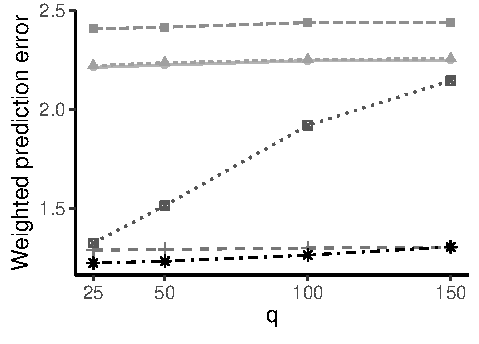
\includegraphics[width=6.9cm]{Plots/NormalHet_qAR1_PredErr_April.pdf} &   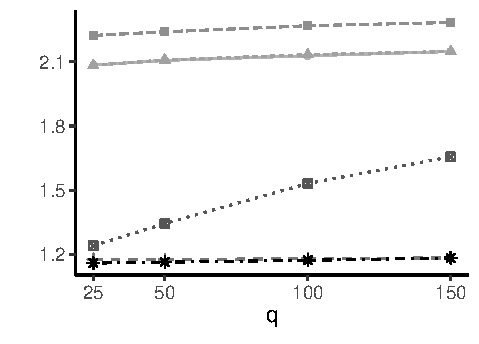
\includegraphics[width=6.9cm]{Plots/NormalHet_qConst_PredErr_April.pdf} &  \\
(c)  & (d)  & \\[6pt]
\end{tabular}
\caption{(a) Model error and (c) weighted prediction error averaged over one hundred independent replications under Model 1 with $q$ varying and $\xi = 0.9$. (b) Model error and (d) weighted prediction error averaged over one hundred independent replications under Model 2 with $q$ varying and $\xi = 0.9$.}\label{fig:q_Results}
\end{figure} 

In Figure \ref{fig:q_Results}, we display average model errors and weighted prediction errors for the settings from Figure \ref{fig:rho_Results}. We observed that when $q \leq 100$, \texttt{MSRL-Val} outperformed all other methods. When $q = 150$, \texttt{MSRL-Val} and \texttt{MRCE-ap} performedvery similarly. It is again worth pointing out that both Model 1 and Model 2 conform to the model assumptions of \texttt{MRCE-ap}, which requires the estimation of as many as $50^2$ more parameters and the selection of two tuning parameters, making \texttt{MRCE-ap} a much more computationally burdensome procedure than \texttt{MSRL-Val}.


\section{Computational details}
\subsection{Derivation of proximal ADMM $\beta$ update}
In this section, we show that 
\begin{align*} \argmin_{\beta \in \mathbb{R}^{p \times q}} & \hspace{5pt}\mathcal{M}_{\rho, \eta}(\beta, \Omega^{(k+1)}, \Gamma^{(k)}; \beta^{(k)}) \\
& = {\rm Prox}_{(\rho \eta)^{-1}\tilde{\lambda} \mathcal{P}} \left\{ \beta^{(k-1)} + \eta^{-1} X'\left(Y + \rho^{-1} \Gamma^{(k-1)} - \Omega^{(k)} - X\beta^{(k-1)}\right)\right\}\\
&  = \argmin_{\beta \in \mathbb{R}^{p \times q}} \left\{ \frac{1}{2}\|\beta -  \beta^{(k-1)} - \eta^{-1} X'\left(Y + \rho^{-1} \Gamma^{(k-1)} - \Omega^{(k)} - X\beta^{(k-1)}\right)\|_F^2 + (\rho \eta)^{-1}\tilde{\lambda} \mathcal{P}(\beta) \right\}.\end{align*}
By construction, 
\begin{align*}
\mathcal{M}_{\rho, \eta}&(\beta, \Omega^{(k+1)},  \Gamma^{(k)}; \beta^{(k)})\\
  & =  \frac{\rho}{2}\|Y + \rho^{-1} \Gamma^{(k-1)} - \Omega^{(k-1)} - X\beta\|_F^2 + \lambda \mathcal{P}(\beta) +  \frac{\rho\eta}{2}\|\beta - \beta^{(k-1)}\|_F^2 \\ 
& \quad \quad - \frac{\rho}{2} {\rm tr}\left[(\beta - \beta^{(k-1)})'X'X(\beta - \beta^{(k-1)}) \right].\\
  \intertext{Then, expanding the first and last terms; and letting $C_1$, $C_2$ and $C_3$ denote constants not depending on $\beta$, }
& = - \rho \hspace{2pt} {\rm tr}\left[(Y + \rho^{-1} \Gamma^{(k-1)} - \Omega^{(k-1)})'X\beta\right] +   \lambda\mathcal{P}(\beta) + \frac{\rho \eta}{2}\|\beta - \beta^{(k-1)}\|_F^2 - \rho \hspace{3pt} {\rm tr}\left[\beta'X'X\beta^{(k-1)}\right] + C_1\\
& = -\rho \hspace{2pt}{\rm tr}\left[\beta'X'(Y + \rho^{-1} \Gamma^{(k-1)} - \Omega^{(k-1)} - X\beta^{(k-1)})\right] + \lambda \mathcal{P}(\beta) + \frac{\rho \eta}{2}\|\beta - \beta^{(k-1)}\|_F^2 + C_1 \\
& \propto - {\rm tr}\left[\eta^{-1} \beta'X'(Y + \rho^{-1} \Gamma^{(k-1)} - \Omega^{(k-1)} - X\beta^{(k-1)})\right] +  \frac{\lambda}{\rho\eta} \mathcal{P}(\beta) + \frac{1}{2}\|\beta - \beta^{(k-1)}\|_F^2 + C_2\\
& = \frac{1}{2} \|\beta - \beta^{(k-1)} - \eta^{-1}X'(Y + \rho^{-1} \Gamma^{(k-1)} - \Omega^{(k-1)} - X\beta^{(k-1)})\|_F^2  +  \frac{\lambda}{\rho\eta} \mathcal{P}(\beta) + C_3, 
\intertext{the desired equality. $\quad\quad \blacksquare$}
\end{align*}

\subsection{Stochastic approximation of the gradient}
Define $\mathcal{H}$ as a randomly selected subset of $\left\{1, \dots, n\right\}$ such that the cardinality of $\mathcal{H}$, ${\rm card}(\mathcal{H})$, is much larger than $q$ but smaller than $n$. Then, let $[Y - X\beta]_{\mathcal{H}}$ and $X_\mathcal{H}$ be the submatrices $Y - X \beta$ and $X$ containing only the rows indexed by $\mathcal{H}$. Similarly let $U_{\mathcal{H}(\beta)} D_{\mathcal{H}(\beta)} V'_{\mathcal{H}(\beta)} = {\rm svd}([Y - X\beta]_{\mathcal{H}})$. Then, we can efficiently approximate the gradient from \eqref{eq:gradient_NN} since, when $n > {\rm card}(\mathcal{H}) \gg q$,
$X'U_\beta V_\beta' \approx X_{\mathcal{H}}'U_{\mathcal{H}(\beta)}V'_{\mathcal{H}(\beta)},$ reducing the per iteration complexity of Algorithm 2 to $O\left\{{\rm card}(\mathcal{H})(q^2 + pq)\right\}$.

\subsection{Method for refitting with unstructured covariance}
To refit the estimators in Section 4.4 (i.e., to obtain the \texttt{-RF} estimates), we use a seemingly unrelated regressions-type penalized normal maximum likelihood estimator. Suppose we are given $\tilde{\beta}$, the estimate of $\beta_*$ from which we want to obtain a refitted version. Define the set $$G(\tilde{\beta}) = \left\{ \beta: \beta \in \mathbb{R}^{p \times q}, \beta_{j,k} = 0 \hspace{5pt} \forall (j,k) \text{ such that } \tilde{\beta}_{j,k} = 0 \right\}.$$ To obtain the refitted version of $\tilde{\beta}$, we solve the following optimization problem: 
\begin{equation}\label{eq:SUR} \argmin_{\beta \in G(\tilde{\beta}), \Omega \in \mathbb{R}^q_+} \left\{n^{-1}{\rm tr}\left[ (Y - X\beta)\Omega(Y - X\beta)' \right] - \log{\rm det}(\Omega) + \frac{\alpha}{2}\|\Omega\|_F^2 \right\},
\end{equation}
where we fix $\alpha = 10^{-4}$. To solve \eqref{eq:SUR}, we use blockwise coordinate descent. Specifically, for $k=1, \dots$, we iterate between the following two steps until convergence: 
\begin{enumerate}
\item $\Omega^{(k+1)} = U \frac{1}{2 \alpha} \left\{ - D + (D^2 + 4\alpha I_q)^{1/2}\right\} U'$ where $n^{-1}(Y - X\beta^{(k)})'(Y - X\beta^{(k)}) = U D U'$ with $U$ orthogonal and $D$ diagonal. 
\item $\beta^{(k+1)} = \argmin_{\beta \in G(\tilde{\beta})} {\rm tr}\left\{(Y - X \beta) \Omega^{(k+1)}(Y - X\beta)' \right\}$
\end{enumerate}
Step 1 is the well known solution for the ridge-penalized normal likelihood precision matrix estimation problem (e.g., see \citet{witten2009covariance}). Step 2 can be solved efficiently using an accelerated projected gradient descent algorithm. We terminate the algorithm when the objective functional value converges. 



% \subsection{Algorithm of \citet{van2016chi2}} 
% The iterates of the algorithm suggested by \citet{van2016chi2} (and the version found in \citet{stucky2017asymptotic}) can be expressed as a fixed-point iteration. In full generality, their algorithm effectively has $(k+1)$th iterate: 
% $$ \beta^{(k+1)} = {\rm Prox}_{\sqrt{n}\lambda \|\tilde{Y} - \tilde{X}\beta^{(k)}\|_* \mathcal{P}} \left[ \beta^{(k)} + \tilde{X}'(\tilde{Y} - \tilde{X}\beta^{(k)}) \right],$$
% where $\tilde{Y} = Y/K$ and $\tilde{X} = X/K$ for some large constant $K$.  


\end{document}

